\documentclass[]{usiinfthesis}

\newcommand{\mynote}[2]{\fbox{\bfseries\sffamily\scriptsize#1}{\small\textsf{\emph{#2}}}\fbox{\bfseries\sffamily\scriptsize}}
%\newcommand{\mynote}[2]{}{}
\newcommand\ar[1]{\mynote{AR}{#1}}

\usepackage{minted}
\usepackage{tabularx}
\usepackage{graphicx}
\usepackage{hyperref}
\usepackage{rotating}
\usepackage{CJKutf8}
\title{Profiling and Analysing Concurrent Libraries\\ on the Java Virtual Machine}
\author{Luca Reina}
\Day{21}
\Month{October}
\Year{2020}
\place{Lugano}
\programDirector{The PhD program Director \emph{pro tempore}}
\begin{committee}
\advisor{Dr.}{Andrea}{Rosà}
\end{committee}
\begin{document}
\maketitle
\frontmatter
\begin{abstract}

\large
Concurrent programming is often used in software applications to enhance performance. Nonetheless, correctly implementing concurrent applications is difficult, especially when it comes to managing mutual exclusion of resources. To ease this task, the Java Class Library (JCL) offers several ready-to-use concurrent libraries. \newline The goal of this dissertation is to create a profiler that can be used to dynamically analyze concurrent applications, collecting data on the usage of concurrent libraries offered by the JCL. \newline First, we analyze the JCL to identify commonly used classes and methods. Then, we design and develop a profiler that relies on DiSL (Domain Specific Language for Instrumentation) and dynamic analysis to instrument the identified classes and methods of interest. The tool is carefully designed to reduce the profiling overhead as much as possible. We apply the profiler on several modern benchmarks, collecting data on the usage of selected methods and classes of interest. Finally, we analyze the obtained results, characterizing the usage frequency of concurrent libraries in modern workloads.
\end{abstract}
\begin{acknowledgements}
\end{acknowledgements}
\tableofcontents
\listoffigures
\listoftables
\mainmatter
\chapter{Introduction}
\large
This chapter introduces the work presented in this thesis dissertation. Section 1.1 illustrates the need for a profiler for concurrent libraries. Section 1.2 introduces the goals and the challenges we faced. Section 1.3 discusses the contribution brought by our work. Finally, Section 1.4 outlines the structure of the dissertation..

\section{Motivation}
For a long time, computation was exclusively sequential, and operations were executed only by single-core processors. Technology was evolving fast, and big leaps forward were achieved almost regularly, producing impactful improvements in the already existing and established architecture. In the early 2000s the focus slowly started shifting as the first multi-core processors began to appear, and concomitant therewith, evolution in technology for single processing units was reaching a peak. 

Nowadays, multi-core architectures represent the norm, and with that, concurrent programming has become fundamental to enhance performance and build competitive software. Nonetheless, writing efficient code that takes proper advantage of this technology is still a complicated -- and sometimes troublesome -- task. Programmers are in fact often on the lookout for simpler and more efficient ways to achieve concurrency, and programming languages generally offer constructs to approach it in a more structured way. 

However, despite the abundance of available libraries, there are very few studies -if none- on the frequency in which they are used. This information may turn out to be very useful in a variety of contexts:

\begin{itemize}
    \item \textit{Compiler development}: having reliable and accurate information about the most used methods and classes of concurrent libraries in modern workloads would give compiler developers the opportunity of focusing on optimizations for such methods, thus creating better performing compilers. %, specifically designed for real usage.
    \item \textit{Libraries implementation}: library implementers would have information about the most used constructs of available concurrent libraries. This data might be used when deciding where to focus their future efforts. For example, improvements could be centered around popular libraries and less on the least used ones. The same libraries could also operate as a blueprint when developing new ones.
    \item \textit{Research}: empirical studies on the usage of libraries are generally welcomed by the research community since they represent accurate information that could be used for future research developments.
\end{itemize}
Yet, to the best of our knowledge, there exist no profilers that can collect this type of information. 

\section{Goals and Challenges}
In this dissertation, we present the design and the development of an accurate and efficient profiler that can collect information on the usage of concurrent libraries included in the Java Class Library (JCL) for software running on the Java Virtual Machine (JVM). Accuracy is ensured through careful implementation, testing, and usage of DiSL, a domain-specific language and framework for bytecode instrumentation. Efficiency is ensured through the DiSL Reflection API, which makes it possible to avoid the usage of expensive runtime checks, the Shadow VM, which allows elaborating the gathered data in a separate JVM and careful instrumentation that makes use of efficient data structures and injects as less code as possible.

Our work faces remarkable challenges. The profiler needs to focus on many different tasks in order to achieve accurate data collection of methods usage frequency. Firstly, the problem of instrumenting \textit{nested method invocations}:  invocations to instrumented methods inside other instrumented methods, thus, methods that aren’t part of the target application code, rather of the source-code implementation of other instrumented methods. If not handled correctly, the profiler will detect calls to libraries done by library code rather than user code, which may be undesirable. Our work identifies where method nesting happens and employs efficient techniques in order to guarantee profiler accuracy. Furthermore, our profiling includes the injection of instrumentation code inside the target application, which may cause measurement perturbation and performance slowdown, if not carefully designed. Our work takes advantage of several techniques to keep data disruption and overhead low, such as profiling techniques, and architectural design choices specifically implemented in order to increase the efficiency and accuracy of the profiler.


\section{Contributions}
To achieve our goal of collecting information on the usage of concurrent libraries made available by the JCL and used by applications running on the JVM, this dissertation makes the following contributions.

\subsection{Analysis}
By carefully analyzing  the JCL, we select all the relevant classes and interfaces representing concurrent libraries, and we divide them into 5 categories, which leads to the definition of as many different profiler modules, named as follows:
\begin{itemize}
    \item \textbf{CCOLL}, focusing on concurrent collections and queues.
    \item \textbf{SCOLL}, focusing on synchronized collections.
    \item \textbf{ELOCK}, focusing on explicit locks.
    \item \textbf{SYNCHRONIZERS}, focusing on synchronizers.
    \item \textbf{FUTURE}, focusing on asynchronous computation.
\end{itemize}
For every selected class, we choose all the major methods of interest. In order to minimize overhead and to avoid introducing unnecessary complexity, we desist from using our profiler to blindly analyze all class methods. Instead, we want to select a smaller, but significant, group of them, leaving out side methods. To accomplish this task, we follow two main criteria: perceived high frequency in usage and structure modification power (i.e. all methods that execute operations of data modification inside the represented structures: creation, deletion, and modification methods).

\subsection{Profiler}
We design and develop an accurate and efficient profiler that can collect information on the usage of concurrent libraries of the JCL for software running on the JVM. The profiler  is composed of three different JVMs running simultaneously and that communicate with one another. [DRAFT] Firstly, the Target Application Server, where the software to be profiled runs.\ar{No. This is the target application (not server) and is the observed application, where the original program + the instrumentation logic run} Then, the DiSL server, which is responsible for out-of-process bytecode instrumentation, thus, for intercepting the loading of specific classes by the target application, and then for injecting them with the instrumentation code as needed. Analysis data is collected inside the target application, which then sends it to the ShadowVM: a third server specifically designed for the analysis operations. This component avoids the injection of analysis code in the target application, which reduces the impact on the target application execution, producing two major benefits: performance improvement and avoidance of possible measurement perturbation due to excessive alteration of the target application code. Based on the architecture, we divide the design of our profiler into four main class modules:
\begin{itemize}
\item \textbf{Instrumentation classes}: they are responsible for defining  instrumentation code. They communicate which classes and methods should be instrumented to the DiSL server, which intercepts specified events occurring in the target applications and injects them with DiSL code snippets. For every method of interest, instrumentation increments a specific thread-local counter, that will be then sent to the analysis server by the Local classes.
\item \textbf{Guard classes}: they are used inside Instrumentation classes and they are responsible for the selection of the instrumentation sites for each method of interest. They also implement the DiSL Reflection API technology, exploiting reflective information of the JCL.
\item \textbf{Local classes}: they implement the profiler logic inside the target application, collecting instrumented data gathered by the Instrumentation classes, in order to then send them to the analysis server.
\item \textbf{Remote classes}: they are responsible for elaborating data collected from the profiling of the target application. They exploit ShadowVM technology, which is a separate virtual machine specifically designed for data analysis.
\end{itemize}

\subsection{Evaluation}
We evaluate the profiler execution on established benchmarks, focusing on the frequency of concurrent method usage and profiler performance. We collect frequency method usage information on concurrent libraries by profiling \textit{Renaissance} \cite{Renaissance}: a well-established benchmark suite containing a range of modern workloads -mainly concurrent- specifically designed for the JVM.This data is, to the best of our knowledge, completely novel. Our analysis shows that the most used libraries are the concurrent collections (CCOLL) and the explicit locks (ELOCK) with overall more than \(5*10^7\) method calls each. Synchronized collections (SCOLL) and asynchronous computation libraries (FUTURE) are far less used, with less than \(8*10^3\) method calls each. A bit more popular, but still much less used in comparison with the first two, are the synchronizers (SYNCHRONIZERS) with less than \(3*10^3\) method usage. In order to ensure efficiency, we also analyse the execution time for each profiler module and none of them scores more than 1,08x of overhead.

\section{Dissertation Outline}
[DRAFT]


\chapter{Background}

[DRAFT: Introdurre Introduzione capitolo]

\section{Bytecode Instrumentation}
\textit{Bytecode instrumentation} is a technique that allows to change the code of compiled class applications. Specifically in Java, it allows to modify the code of \textit{.class} files produced by the Java Compiler. It can be achieved in three different ways:
\begin{itemize}
    \item \textbf{At Compile-Time:} It is simplest way to implement it, and it is achieved by adding instrumentation to classfiles before the application is run. However, it may be wastful, instrumenting many unused classes, and it can only focus on classes available at compile-time.
    \item \textbf{At Load-Time:} It is achieved by injecting instrumentation code inside loaded classfiles before linking. There are two types:
    \begin{itemize}
        \item \textbf{In-Process}: it is executed inside the target application, and it allows to instrument all loaded classes. However it may cause \textit{infinite instrumentation recursion}, when instrumenting a construct with an injection of the same construct (e.g. We're instrumenting all \textit{System.out.println} method of a certain class, printing a message every time we encounter this instruction. In order to do so, we inject all methods with another \textit{System.out.println}. However, these methods will not be excluded from the analysis. Thus, They will be injected with another \textit{System.out.println}, which, in turn, will be also instrumented, creating an infinite stream of instrumentation recursion). Since instrumentation to the JCL might create this type of problem, it is often excluded, limiting bytecode coverage. it also might cause interference with JVM initialization or class loading.
        \item \textbf{Out-Of-Process:} It is the most difficult to implement, but it also the most beneficial. It tackles the infinite instrumentation recursion problem, while allowing \textit{full bytecode coverage}, ergo, the possibility to instrument the JCL. Access to reflective information of the loaded classes might be limited. However, successful attempts to overcome this problem have been made.
    \end{itemize}
\end{itemize}


\section{AOP: Aspect-Oriented Programming}
Bytecode Instrumentation is often used in \textit{aspect-oriented programming} to implement \textit{aspects} into the code, which are features added to specific parts of a software. This programming paradigm doesn't aim to introduce new functionalities -even though it potentially could-, rather to trace program behaviours or properties, augmenting them only temporarily.


\section{Dynamic Analysis}
\textit{Dynamic Analysis} is a programming technique that aims to evaluate programs during their execution, rather than examining code statically. It can be used for a multitude of software engineering purposes: software testing, profiling, debugging, and reverse engineering. It's strengths reside in the usage of real data to asses software functionalities and performance deficiencies, gathering information that otherwise would be nearly impossible to get with static approaches. 

\section{DiSL}

\textit{DiSL} (\textbf{D}omain \textbf{S}pecific \textbf{L}anguage for \textbf{i}nstrumentation) is a domain-specific language designed for out-of-process bytecode instrumentation, that relies on AOP principles to allow efficient and accurate implementation of dynamic analysis mechanisms for Java applications. DiSL instrumentation code is written through code snippets, which are structured with two major constructs. Firstly, \textbf{instrumentation site} which specifies the code location of target applications, where instrumentation code will be injected. It can be described through:
\begin{itemize}
    \item \textit{Annotations}: to specify the type and the timing of the snippet. For example to indicate that the instrumentation will be injected before or after a specific bytecode instruction.
    \item \textit{Markers}: to allow access to specific classfiles code regions. For example to mark precise bytecode instructions or the body of an indicated method.
    \item \textit{Scopes}: to allow specification of constructs name. For example to indicate the precise name of a method to be instrumented from a specific class. 
    \item \textit{Guards}: to allow further filtering through static analysis executed at weave-time.
\end{itemize}
Secondly, \textbf{instrumentation code} which are instantiated and inlined in the correspondent instrumentation sites and they may:
\begin{itemize}
    \item \textit{Access Synthetic Local Variables}: to allow passage of data through instrumentation sites.
    \item \textit{Access Static Context information}: to allow information access to data collected at instrumentation time, such as method or class names, signatures, visibility, etc.
    \item \textit{Access Dynamic Context information}: to allow information access to data collected at runtime, such as method argument values, local variable values, class instance, etc.
\end{itemize}

\subsection{DiSL Reflection API}
As previously discussed, DiSL relies on an out-of-process bytecode instrumentation architecture, which means that instrumentation will be injected from the DiSL server to the JVM of the target application. This type of engineering doesn't ensure by default, complete reflective information of loaded classes. It allows, in fact, to instrument objects of the target class or objects that are direct subtypes of the target class. This excludes every class that is an indirect subtype of the target class. For example, if we wanted to instrument -without reflective information- the method \textit{clear} of the \textit{java.util.Map} interface and all of its inheriting classes, we would automatically be instrumenting also the same method for the \textit{java.util.ConcurrentMap} interface, since it extends directly the \textit{java.util.Map} interface. However, if we wanted to also instrument the same method in the class \textit{java.util.ConcurrentHashMap}, which implements \textit{java.util.ConcurrentMap}, we would need to use very expensive dynamic checks. Thus, it would still be possible to pursue an accurate analysis, however, it would cost us important resources in terms of performance and time.

\textbf{DiSL Reflection API} solves this problem. It is a technology utilized by DiSL that provides reflective information about the supertypes of the classes under instrumentation. So that, once the JVM starts, it is possible to build the correct class parentage, avoiding usage of expensive runtime checks, otherwise necessary in an out-of-process bytecode instrumentation architecture.

\subsection{Shadow VM}

DiSL, as described so far, allows out-of-process bytecode instrumentation. Therefore, every code snippet inlined into the target application runs inside the target application JVM itself. Even though it actually is the ultimate goal of this architecture, it still exhibits two major problems:
\begin{enumerate}
    \item \textit{Reduced performance}: Introducing new instructions inside an application will necessarily weight down program execution time, consequently increasing the overhead.
    \item \textit{Potential data disruption}: time is not the only resource impacted when a software is augmented with new instructions. Memory usage also changes. Therefore, program behaviour may suffer inadvertently of modification as well, which may result in data inaccuracy and consequently in incorrect analyses.
\end{enumerate}

In order to mitigate these complications, DiSL offers the possibly to utilize the \textbf{Shadow VM}, which is an additional Java Virtual Machine, introduced to separate the process of gathering data, with the actual analysis. With this technology, instrumentation code snippets injected and run into the target application JVM, are responsible only for the collection of the needed information. Then, through the APIs offered by DiSL, this data is sent to the ShadowVM, where it is organized and analysed as desired. 

This type of approach significantly reduces overhead and data disruption, while also improving:
\begin{enumerate}
    \item \textit{Isolation}: since it avoids, as much as possible, sharing state with the target application. 
    \item \textit{Separation of concerns}: since analyses and data gathering can be built separately, which is also rationally a better solution.
\end{enumerate}

\section{Libraries}
As mentioned in the introduction, the profiler targets concurrent structures of the JCL, dividing the focus on 5 different modules. This section is not meant to be a detailed list of analysed classes and methods, but rather an explanation on the reasoning behind the grouping and an introductory description of every single module. Further classifications will be discussed in chapter [DRAFT].

\subsection{Synchronized Collections}
Since Java 2, the JCL offered the \textit{Collections framework} which is a set of classes and interfaces that allows implementation and manipulation of commonly reusable data structures, such as lists, sets, maps, etc. Although concurrent programming with this type of data structures is possible, it can also result in an intimidating and error-prone task. In order to ease this job, Java introduced over the years new constructs that implicitly ensures thread-safety, sparing programmers to do it themselves. Synchronized collections are a prime example of this concept. They are synchronization wrappers for standard collections: a group of 6 static methods of the \textit{Collections} class, that receive in input standard data structure objects, returning thread-safe collections. Synchronization is ensured with intrinsic locking, which enforces exclusive access to the wrapped collections. Data consistency/integrity is assured, but with a possible penalty in performance.

\noindent
We decided to group this type of classes together in order to build a specific profiler module called SCOLL.

\subsection{Concurrent Collections and Queues}
Another example of constructs introduced to ensure thread-safety are concurrent collections. They were added with the launch of Java 5, and more specifically of the \textit{java.util.concurrent} library, where the collection framework has been expanded in order to fit the new concurrent architectures, introducing specific collection implementations, designed to be used in multi-threaded contexts. Compared with the synchronized collections, the main differences reside in the following two areas of interest:
\begin{enumerate}
    \item \textit{Architecture}: while synchronized collections are static wrapper methods of a single class, concurrent collections are a list of classes and interfaces. Thus, programmers are able manipulate the latter, expanding and implementing them, increasing customization opportunities. However, programmers familiarity with concurrent collections methods might not be immediate, since they might differ from the ones of the standard library. This is not the case with synchronized collections, since they return the same standard objects, but wrapped to ensure thread-safety.  
    \item \textit{Behaviour}: contrary to synchronized collections, that ensure thread-safety by enforcing exclusive access through intrinsic locking, concurrent collections divide data structures into segments, allowing access accordingly. Thus, multiple threads can access the same collection at the same time. Depending on the implementation requirement, the library usage choice should be done accordingly.
\end{enumerate}

\noindent
We decided to group this type of classes together in order to build a specific profiler module called CCOLL.


\subsection{Synchronizers}
Another framework introduced with the \textit{java.util.concurrent} package is defined as Synchronizers. It is a collection of five concrete classes representing common mechanisms for managing synchronization, locking of threads and queuing automatically. They vary according to the number of states managed by the class: exclusive states versus shared states.

\noindent
We decided to group this type of classes together in order to build a specific profiler module called SYNCHRONIZERS.


\subsection{Explicit Locks}
Another way to represent synchronization can be found inside the \textit{java.util.concurrent} package, where a subpackage named \textit{locks} is located. It is a framework that can be used to explicitly represent operations such as locking and waiting for conditions. It differs from the common \textit{synchronization} block since it gives much more flexibility, at the cost of a more complex and awkward syntax. The main differences are:
\begin{enumerate}
    \item While a synchronized block is contained inside a method, explicit locks operations (i.e. \textit{lock()}, \textit{unlock()}, etc.) can be managed in different methods.
    \item Explicit locks allow the usage of \textit{fairnes}, while synchronized blocks don't.
    \item The explicit locks framework offers methods for lock acquiring operations that reduce thread blocking time (i.e. \textit{tryLock()}).
    \item In a synchronized block a waiting thread can't be interrupted, while explicit locks offer methods to accomplish this task (i.e. \textit{lockInterruptibly()})
\end{enumerate}

\noindent
We decided to group this type of classes together in order to build a specific profiler module called ELOCKS.

\subsection{Future}
The last framework we decided to add to the profiler was the Future interface and relative subclasses. They are used in contexts of asynchronous computation and -in particular- when waiting for the results. In the case of heavy operations, that require a long time to complete, it is possible to use futures to encapsulate future results of these operations, allowing to continue execution of other operations, while waiting for the heavy task to complete.

\noindent
We decided to group this type of classes together in order to build a specific profiler module called FUTURE.

\chapter{State of the Art}
In this chapter we compare our work with the current state of the art. Section 3.1 showcases a variety of parallel profilers, highlighting their strengths and weaknesses. Section 3.2 discusses the contributions that our tool provides in comparison with the profilers presented in Section 3.1.

\aar{I don't think you should call them "parallel profilers". They are "profiler for concurrent applications". Keep in mind that concurrency and parallelism are different concepts. In Java you can develop concurrent applications, not parallel. Please change the chapter}

\section{Parallel Profilers}
Several tools have been developed over the years to achieve dynamic profiling of applications running on the JVM. Many of them focuses on various aspects of concurrency, such as thread and lock profiling and errors and performance inefficiencies detection.

Iceberg \cite{Iceberg} is a tool designed for locating potential software hangs while using synchronized methods in Java applications\ar{You mean, deadlock?}. It works by recording all synchronized method calls at runtime, and then highlighting outliers\ar{It is not clear what "outlier" means here. Shouldn't it detect deadlocked threads (based on the information that you wrote above?}. The final objective of this profiler is to pinpoint potential performance inefficiencies.

Chappie \cite{Chappie} focuses on energy accounting for Java applications. It allows the analysis of the energy consumption of all application logical units (i.e. methods, classes, packages, etc.), by producing an analyzable energy footprint. However, it doesn't specifically target concurrency.

Heijo \cite{Heijo} is a profiler specifically designed to improve software performance, by visualizing program execution as a three-dimensional software city\ar{city, really?}. Each package, class and method of a running Java application is represented as a block, which size is defined by execution time. The longer the time, the higher the block. However, it doesn't specifically target concurrency. \ar{I would not include profilers not targeting concurrency. They are out of the scope here. Moreover it is not clear in which conference it was published (the name is in Japanese!)}

Kremlin \cite{Kremlin} is a profiler that focuses on identifying target application regions where implementing concurrency techniques may better performance during program execution. 

jPredictor \cite{jPredictor} focuses on concurrency errors for Java application. It works by instrumenting programs at runtime and producing resulting traces of relevant events. The latter is\ar{are?} then statically analyzed, providing concurrency errors predictions.

Free Lunch \cite{FreeLunch} is a tool specifically designed for lock profiling on Java Server application. It focuses on performance issues caused by parallel execution phases where the thread progress is impended by locks. In order to keep the overhead low, it relies on statistical sampling, which may deeply impact tool accuracy. \ar{You also detect locks. Does this profiler detect implicit or explicit locks? If only implicit, then your profiler is complimentary to this one (you target only explicit locks)}

HPCToolkit \cite{HPCToolkit} is a tool suite specifically designed to pinpoint and quantify bottlenecks that may happen during the execution of parallel programs. Thus, it aims to improve overall applications performance.

THOR \cite{THOR} is a profiler that focuses on thread state, providing information about thread idling and execution. However, tool overhead and consequent measurement perturbation may be very high, thus allowing accurate and efficient profiling only for small periods of time.

Other profilers that focus on analyzing concurrency for Java software applications are YourKit \cite{YourKit}, Health Center \cite{Health Center}, vTune Amplifier \cite{vTune Amplifier}, JProfiler \cite{JProfiler}, and Mission Control \cite{Mission Control}. They all focus on common analyses for monitoring and profiling of memory utilization. \ar{Please make sure that they target concurrent applications.}


\section{Contribution} 
In the previous section, we described prevailing profilers that analyze concurrency for applications running on the JVM. They all aim to improve error and performance inefficiencies, focusing on aspects such as thread and lock usage, thread state, bottlenecks, and concurrency errors. However, none of them analyzes method and class usage frequencies for concurrent libraries of the JCL.

Thus, our profiler provides a completely novel point of view. To the best of our knowledge, the profiler presented in this dissertation is the first tool specifically designed for analysing usage frequencies of concurrent libraries provided by the JCL in applications running on the JVM.




\chapter{Analysis}
In this chapter we discuss the process that we followed in order to create a selection of classes and methods onto which we ran the analysis. It is divided in 2 main sections. In the first one we explain the grouping and the class selection, while in the second one the method filtering for every selected class.


\section{Class Selection \& Grouping}
The class selection process is necessarily deep rooted in the task that this profiler wants to achieve: analyse and profile concurrent libraries for the JCL. First of all, we researched what are the most popular frameworks used when programming in a concurrent environment. This operation involved a mix of searching the web and looking through manuals that tackle the topic. We achieved to collect the 5 main topics already  discussed in the background chapter: synchronized collections, concurrent collections, explicit locks, synchronizers, and future. After this first effort, we focused on the official Java documentation offered by Oracle, and for every group we gathered all the classes that we deemed to be suitable for the analysis. Then we arranged them in order to recreate the Java hierarchy. Operation that we purposely conducted to achieve proper documentation, but also to ease implementation and utilize the DiSL Reflection API. Further discussions on this topic will be expressed in detail in chapter 4. In the following pages we describe the classes choice group by group.

\subsection{Synchronized Collections}
As previously discussed in the background chapter, the synchronized collections framework is an assortment of wrappers that ensures thread-safety when using standard collections in a concurrent environment. The structure is pretty straight-forward, with only one class offering several public and static methods to achieve synchronization: \textit{Collections}. From an outside perspective there are no practical differences when using synchronized collections rather than standard collections. However, if we take a look at the code, we can see that these synchronized collections are actually represented inside the Collections class as a list of static classes with default -or sometimes private- visibility. For this particular reason, they could be used inside applications, thus we decided to also profile them and the complete list of classes is the following:

\begin{itemize}
    \item Collections
    \begin{itemize}
        \item SynchronizedCollection 
        \item SynchronizedList 
        \item SynchronizedMap 
        \item SynchronizedSortedMap
        \item SynchronizedNavigableMap
        \item SynchronizedSet
        \item SynchronizedSortedSet
        \item SynchronizedNavigableSet
    \end{itemize}
\end{itemize}


\subsection{Concurrent Collections}
The concurrent collections framework is, as previously discussed in the background chapter, an extension of the \textit{Collection} framework provided by the \textit{java.util} package. It offers many new data structures adapted to work in a concurrent environment. It is structured on two main interfaces: BlockingQueue and ConcurrentMap. Both constructs are the synchronized version of the interfaces Queue and Map respectively, and both implement them. All the other constructs of the framework are either descending interfaces with specializing qualities (e.g. BlockingDeque, ConcurrentNavigableMap, etc.), or concrete classes implementation of the two main interfaces just discussed (e.g. ArrayBlockingQueue, ConcurrentHashMap, etc.).  In addition, there are three other classes that implement neither of the two main interfaces, nor descendant of them. They are the: CopyOnWriteArrayList representing a concurrent version of an List, and CopyOnWriteArraySet and ConcurrentSkipListSet representing two different ways to implement a concurrent version of a Set. 

The complete list of classes is the following:

\begin{itemize}
    \item \textbf{Interfaces:}
    \begin{itemize}
        \item BlockingQueue<E>
        \begin{itemize}
            \item BlockingDeque<E>
            \item TransferQueue<E>
        \end{itemize}
        \item ConcurrentMap<K,V>
        \begin{itemize}
            \item ConcurrentNavigableMap<K,V>
        \end{itemize}
    \end{itemize}
    \item \textbf{Classes:}
    \begin{itemize}
        \item CopyOnWriteArrayList<E>
        \item CopyOnWriteArraySet<E>
        \item ConcurrentSkipListSet<E>
    \end{itemize}
    \textit{Implementing BlockingQueue<E>:}
    \begin{itemize}
        \item ArrayBlockingQueue<E>
        \item DelayQueue<E extends Delayed>
        \item LinkedBlockingQueue<E>
        \item PriorityBlockingQueue<E>
        \item SynchronousQueue<E>
    \end{itemize}
    \textit{Implementing BlockingDeque<E>:}
    \begin{itemize}
        \item LinkedBlockingDeque<E>
    \end{itemize}
    \textit{Implementing TransferQueue<E>:}
    \begin{itemize}
        \item LinkedTransferQueue<E>
    \end{itemize}
    \textit{Implementing ConcurrentMap<K,V>:}
    \begin{itemize}
        \item ConcurrentHashMap<K,V>
    \end{itemize}
    \textit{Implementing ConcurrentNavigableMap<K,V>:}
    \begin{itemize}
        \item ConcurrentSkipListMap<K,V>
    \end{itemize}
\end{itemize}


\subsection{Explicit Locks}
The explicit locks framework, as previously discussed in the background chapter, is a collection of constructs that allows to explicitly represent operations such as locking and waiting for condition. It is structured on thre main interfaces:
\begin{enumerate}
    \item \textbf{Lock:} As the name suggests, this interface represents a lock, and offers several methods to grant thread-safety when accessing shared resources. Compared to the implicit locking structure utilized by the synchronized collections framework, it endows more flexibility, allowing locks to be acquired and released in separate scopes, and not in a block structured way.  
    \item \textbf{ReadWriteLock:} this interface represents a pair of locks designed to grant thread-safety while separating access operations on a shared resources: a lock is used for reading and the other one for writing. Compared to the Lock interface, that indistinctly allows exclusive access to the resource, ReadWriteLock grants multiple access when reading, while writing is still exclusive.
    \item \textbf{Condition:} When an explicit lock replaces the usage of synchronized blocks, this Condition interface is used in order to represent monitor methods (i.e. \textit{wait()}, \textit{notify()}, and \textit{notifyAll()}). Compared with the latter, conditions offer more flexible operations, such as the possibility to guarantee ordering of notification, or not having the necessity of holding a lock when performing notifications.
\end{enumerate}

\noindent
In addition to these three interfaces, and the two classes implementing them: ReentrantLock and ReentrantReadWriteLock, there are also three other main classes in the package:

\begin{enumerate}
    \item \textbf{AbstractOwnableSynchronizer:} It is an abstract class that offers a structure designed to be used to create custom synchronizes (e.g. semaphores, phasers, etc.). It could have been made part of the synchronizers module, but since it is found in the \newline \textit{java.util.concurrent.locks} package, and since it strongly makes use of locking structures, we opted for keeping it separate. 
    \item \textbf{LockSupport:} As the name suggests, it a support class that facilitate the creation of locks and other synchronizations structures, providing basic thread blocking primitives. 
    \item \textbf{StampedLock:} A capability-based lock class granting three methodologies for controlling access of shared resources: read, write, and optimistic reading. It doesn't implement neither of the two main lock interfaces previously discussed, rather it offers methods that create the possibility to be seen as either one of them.
\end{enumerate}

\noindent
For the explicit locks framework we selected and organized the classes as follows:

\begin{itemize}
    \item \textbf{Interfaces:}
    \begin{itemize}
        \item Lock
        \item ReadWriteLock
        \item Condition
    \end{itemize}
    \item \textbf{Abstract Classes:}
    \begin{itemize}
        \item AbstractOwnableSynchronizer
        \begin{itemize}
            \item AbstractQueuedSynchronizer
            \item AbstractQueuedLongSynchronizer
        \end{itemize}
    \end{itemize}
    \item \textbf{Classes:}
    \begin{itemize}    
        \item LockSupport
        \item StampedLock
    \end{itemize}
    \textit{Implementing Lock:}
    \begin{itemize}
        \item ReentrantLock
    \end{itemize}
    \textit{Implementing ReadWriteLock:}
    \begin{itemize}
        \item ReentrantReadWriteLock
    \end{itemize}
\end{itemize}

\subsection{Synchronizers}
As previously discussed in the background chapter, the synchronizers framework is a collection of five concrete classes representing common mechanisms for automatically managing synchronization, locking of threads and queuing.

\noindent
For the synchronizers framework we selected and organized the classes as follows:

\begin{itemize}
    \item Semaphore
    \item CountDownLatch
    \item CyclicBarrier
    \item Phaser
    \item Exchanger<V>
\end{itemize}

\subsection{Future}
As previously discussed in the background chapter, the future frameworks provides constructs to encapsulate future results of heavy asynchronous operations, while allowing to continue execution of other operations. The main interface is Future, and exaclty represents this concept. Other constructs are descending interfaces or implementing classes of it.

\noindent
For the future framework we selected and organized the classes as follows:

\begin{itemize}
    \item \textbf{Interfaces:}
    \begin{itemize}
        \item Future
        \begin{itemize}
            \item Response<V>
            \item RunnableFuture<V>
            \item ScheduledFuture<V>
            \begin{itemize}
                \item RunnableScheduledFuture
            \end{itemize}
        \end{itemize}
    \end{itemize}
    \item \textbf{Classes:}
    \newline
    \textit{Implementing RunnableFuture<T>:}
    \begin{itemize}
        \item FutureTask<T>
    \end{itemize}
    \textit{Implementing Future<V> \& CompletionStage<T>:}
    \begin{itemize}
        \item CompletableFuture<V>
    \end{itemize}
\end{itemize}


\section{Methods Selection}
After collecting all the necessary classes for the analysis, our focus then shifted on methods selection. We had two options:
\begin{enumerate}
    \item Blindly analyse all methods offered by the chosen classes.
    \item Select a smaller, significant group of methods.
\end{enumerate}
 The first option would have made the analysis phase a lot faster, basically skipping methods selection completely. However the profiler weight would have been significant, and when run onto target applications, it would have resulted in poorer performance and heavier overhead. In addition, implementation phase would have been more time consuming. On the contrary, with the second option, we would have had to invest a lot more time and effort into the analysis phase, yet earning a better performing profiler. We analysed pros and cons of both options and our choice was made once again reflecting on the reasoning behind the tool: to give programmers a realistic look inside the concurrent aspect of the JCL, offering useful information about the usage of those libraries. In our opinion, it would have been pointless to provide data on every single method, when a significant group of them are typically not used, or bring little, to no information at all. Especially when at the expenses of the performance. For this particular reason we decided to go with the second option.
 
\subsection{Filtering Criteria}
 Method selection occupies a prominent portion of the analysis phase. The goal of this process is to select the right amount of methods, preventing overfilling, while still achieving a successful filtering, thus avoiding to leave out fundamental operations. To achieve this task, we based method selection on two main criteria:
 \begin{itemize}
    \item \textbf{Methods structure modification power: } When talking about concurrent data structure, which in our analysis are represented with the concurrent collections and synchronized collections modules, we selected all the methods that provide modification to the actual structures:
    \begin{itemize}
        \item \textit{Insertion methods}: such as \textit{push()}, \textit{put()}, and \textit{addAll()}. Methods that provide elements inclusion inside collections.
        \item \textit{Modification methods}: such as \textit{compute()}, \textit{replace()}, and \textit{replaceAll()}. Methods that provide elements manipulation inside collections.
        \item \textit{Removal methods}: such as \textit{delete()}, \textit{clear()}, and \textit{drainTo()}. Methods that provide elements deletion inside collections.
    \end{itemize}
    For the remaining modules we selected methods that were structurally important, representing core functionalities of the classes. For example, for the explicit locks and synchronizers modules, we picked methods such as \textit{lock()}, \textit{unlock()}, \textit{acquire()} and \textit{await()}, and for the future module, methods like \textit{cancel()}, \textit{run()} and \textit{complete()}. 
    
    \item \textbf{Methods perceived high frequency in usage: }However, not all methods that modify concurrent data structures or that are structurally of importance, are frequently used methods. Reading operations such as getters, and iterative functions such as \textit{forEach()}, are also widely used and provide important information. Thus, we decided to also select this type of methods and implement them into the analysis. 
 \end{itemize}
 \noindent
 Examples of methods we decided to leave out from the final listing are: \textit{toString()}, \textit{containsKey}, \textit{hashCode}, \textit{isEmpty()}, and \textit{size()}. Thus, all methods that return information on the state or content of the structures, besides getters.
 
 
 \subsection{Methods Grouping}
 In order to understand the reasoning behind this section, it is important to also know what the final product of running the profiler onto target applications will look like. Further and more detailed explanations will be done in the following chapters. When run, the tool will produce in output data, in the form of counters, for every selected method.
 
 In order to provide a useful analysis and to simplify reading of the final product produced by the profiler, we decided to merge together particular methods. The process followed two main criteria:
 \begin{itemize}
     \item \textbf{Overloading methods: }all the methods with the same name, but different attributes. For example, methods such as:
     \begin{itemize}
         \item boolean offer(E e)
         \item boolean offer(E e, long timeout, TimeUnit unit)
     \end{itemize}
     We made this choice in order to build a profiler that provides information of what method is being used, and not about the specific type of implementation.
 \end{itemize}
 \begin{itemize}
     \item \textbf{Specializing methods: }all the methods that achieve the same conceptual task, but specialize behaviours without necessarily exploiting overloading. For example, methods such as:
     \begin{itemize}
         \item static void park()
         \item static void park(Object blocker)
         \item static void parkNanos(long nanos)
         \item static void parkNanos(Object blocker, long nanos)
         \item static void parkUntil(long deadline)
         \item static void parkUntil(Object blocker, long deadline)
     \end{itemize}
     We made the choice to merge all these methods in only one counter for the same reason as before. We aimed to build a profiler that provides information of what method is being used, and not the specific type of implementation.
 \end{itemize}
 
 \noindent
 It is important to mention that methods that achieve the same results, but are conceptually slightly different (e.g. \textit{put()} and \textit{add()} of the \textit{BlockingQueue} interface) were not merged together. The reasoning behind this choice is actually the same as before: we aimed to build a profiler that provides information of what method is being used. Even though one could argue that this choice could increase redundancy of information, merging this kind of methods would have made -in our opinion- the analysis too generic, thus not actually useful.
 
 \subsection{Nested Methods}
 Another aspect that will be further explored in the following chapters, that however impacted the analysis, is the nested methods concept. For every method of interest, we had to look at the official implementation, and check if other methods of interest were used inside of them.
 
 \noindent
 An example of this concept is represented in the following code:
 
\begin{minted}[linenos]{java}
public boolean add(E e) {
    return al.addIfAbsent(e);
}
\end{minted}

\noindent
 It is the implementation of the method \textit{add} of the \textit{CopyOnWriteArraySet} class. It uses the \textit{addIfAbsent} method of the same class (line 2), which is also part of the analysis. This poses a problem since, during the profiling of targets applications, every time an \textit{add} method would be instrumented, the \textit{addIfAbsent} method would be as well, invalidating final results. Solution and further explanation of this issue are discussed in the implementation chapter, but in order to check if the solution was actually working, we had also to draw up a list of nested methods during the analysis.
 
 \noindent
 It is important to mention that nested methods refer only to method of the same module.
 
 \subsection{Method of Interest Listing}
 Here we list all the method of interest selected for the analysis divided by module and class. Methods grouped together are specified in the same list element, while nested methods are represented with the $\Rightarrow$ symbol under the implementing method.
 
\subsubsection{Synchronized Collections}

\small{
\noindent
\textbf{Collections:}
\begin{itemize}
    \item   static <T> Collection<T> synchronizedCollection(Collection<T> c)
    \item   static <T> List<T> synchronizedList(List<T> list)
    \item   static <K,V> Map<K,V> synchronizedMap(Map<K,V> m)
    \item   static <K,V> NavigableMap<K,V> synchronizedNavigableMap(NavigableMap<K,V> m)
    \item   static <T> NavigableSet<T> synchronizedNavigableSet(NavigableSet<T> s)
    \item   static <T> Set<T> synchronizedSet(Set<T> s)
    \item   static <K,V> SortedMap<K,V> synchronizedSortedMap(SortedMap<K,V> m)
    \item   static <T> SortedSet<T> synchronizedSortedSet(SortedSet<T> s)
\end{itemize}

\noindent
\textbf{SynchronizedCollection:}
\begin{itemize}
    \item   boolean add(E e)
    \item   boolean remove(Object o)
    \item   boolean addAll(Collection<? extends E> coll)
    \item   boolean removeAll(Collection<?> coll)
    \item   boolean retainAll(Collection<?> coll)
    \item   void clear()
    \item   void forEach(Consumer<? super E> consumer)
    \item   boolean removeIf(Predicate<? super E> filter)
\end{itemize}

\noindent
\textbf{SynchronizedList:}
\begin{itemize}
    \item   E get(int index)
    \item   E set(int index, E element)
    \item   void add(int index, E element)
    \item   E remove(int index)
    \item   void replaceAll(UnaryOperator<E> operator)
\end{itemize}

\noindent
\textbf{SynchronizedMap:}
\begin{itemize}
    \item  V get(Object key)
    \item  V getOrDefault(Object k, V defaultValue)
    \item  V put(K key, V value)
    \item  V remove(Object key)
    \mbox{}\\  boolean remove(Object key, Object value)
    \item  void putAll(Map<? extends K, ? extends V> map)
    \item  void clear()
    \item  void replaceAll(BiFunction<? super K, ? super V, ? extends V> function)
    \item  V putIfAbsent(K key, V value)
    \item  boolean replace(K key, V oldValue, V newValue)
    \mbox{}\\  V replace(K key, V value)
    \item  void forEach(BiConsumer<? super K, ? super V> action)
    \item  V computeIfAbsent(K key,Function<? super K, ? extends V> mappingFunction)
    \item  V computeIfPresent(K key,BiFunction<? super K, ? super V, ? extends V> remappingFunction)
    \item  V compute(K key, BiFunction<? super K, ? super V, ? extends V> remappingFunction)
    \item  V merge(K key, V value, BiFunction<? super V, ? super V, ? extends V> remappingFunction)
\end{itemize}

\noindent
\textbf{SynchronizedSortedMap:}
\begin{itemize}
    \item  K firstKey()
    \item  K lastKey()
\end{itemize}

\noindent
\textbf{SynchronizedNavigableMap:}
\begin{itemize}
    \item  Entry<K, V> lowerEntry(K key)
    \mbox{}\\  K lowerKey(K key)
    \item  <K, V> floorEntry(K key)
    \mbox{}\\  K floorKey(K key)
    \item  Entry<K, V> ceilingEntry(K key)
    \mbox{}\\  K ceilingKey(K key)
    \item  Entry<K, V> higherEntry(K key)
    \mbox{}\\  K higherKey(K key)
    \item  Entry<K, V> firstEntry()
    \item  Entry<K, V> lastEntry()
    \item  Entry<K, V> pollFirstEntry()
    \item  Entry<K, V> pollLastEntry()
\end{itemize}

\noindent
\textbf{SynchronizedSortedSet:}
\begin{itemize}
    \item  E first()
    \item  E last()
\end{itemize}

\noindent
\textbf{SynchronizedNavigableSet:}
\begin{itemize}
\item  E lower(E e)
\item  E floor(E e)
\item  E ceiling(E e)
\item  E higher(E e)
\item  E pollFirst()
\item  E pollLast()
\end{itemize}





\subsubsection{Concurrent Collections}




\noindent
\textbf{BlockingQueue<E>:}
\begin{itemize}
    \item boolean add(E e)
    \item int drainTo(Collection<? super E> c, int maxElements)
    \mbox{}\\ int drainTo(Collection<? super E> c)
    \item boolean offer(E e)
    \mbox{}\\ boolean offer(E e, long timeout, TimeUnit unit)
    \item E poll(long timeout, TimeUnit unit)
    \mbox{}\\ E poll()
    \item void put(E e)
    \item boolean remove(Object o)
    \item E take()
    \item void clear() 
\end{itemize}

\noindent
\textbf{BlockingDeque<E>:}
\begin{itemize}
    \item boolean offerFirst(E e)
    \mbox{}\\ boolean offerFirst(E e, long timeout,TimeUnit unit)
    \mbox{}\\ $\Rightarrow$   void addFirst(E e)
    \mbox{}\\ $\Rightarrow$   void push(E e)
    \item boolean offerLast(E e) 
    \mbox{}\\boolean offerLast(E e, long timeout,TimeUnit unit)
    \mbox{}\\ $\Rightarrow$   boolean offer(E e)
    \mbox{}\\ $\Rightarrow$   boolean offer(E e, long timeout, TimeUnit unit)
    \mbox{}\\ $\Rightarrow$   void addLast(E e)
    \mbox{}\\ $\Rightarrow$   add(E e)
    \item void putFirst(E e)
    \item void putLast(E e)
    \mbox{}\\ $\Rightarrow$   void put(E e)
    \item E takeFirst()
    \mbox{}\\ $\Rightarrow$   E take()
    \item E takeLast() 
    \item E pollFirst(long timeout, TimeUnit unit)
    \mbox{}\\ E pollFirst()
        \mbox{}\\ $\Rightarrow$   E removeFirst()
        \mbox{}\\ $\Rightarrow$   E pop()
        \mbox{}\\ $\Rightarrow$   E remove()
        \mbox{}\\ $\Rightarrow$   E poll()
        \mbox{}\\ $\Rightarrow$   E poll(long timeout, TimeUnit unit)
    \item E pollLast(long timeout, TimeUnit unit)
        \mbox{}\\ E pollLast()
        \mbox{}\\ $\Rightarrow$   E removeLast()
    \item boolean removeFirstOccurrence(Object o)
    \mbox{}\\ $\Rightarrow$   boolean remove(Object o)
    \item boolean removeLastOccurrence(Object o)
        \item E getFirst()
        \item E getLast()
\end{itemize}

\noindent
\textbf{TransferQueue<E>:}
\begin{itemize}
    \item void transfer(E e)
    \item boolean tryTransfer(E e)
    \mbox{}\\ boolean tryTransfer(E e, long timeout, TimeUnit unit)
\end{itemize}

\noindent
\textbf{ArrayBlockingQueue<E>:}
\begin{itemize}
    \item   int drainTo(Collection<? super E> c)
    \mbox{}\\   int drainTo(Collection<? super E> c, int maxElements)
    \mbox{}\\ $\Rightarrow$   add(E e)                \textit{Collection}
    \mbox{}\\ $\Rightarrow$   drainTo(Collection<? super E> c, int maxElements)
    \item   boolean add(E e)
    \mbox{}\\ $\Rightarrow$   add(E e)                \textit{AbstractQueue}
    \mbox{}\\ $\Rightarrow$   offer(E e)        \textit{Queue}
\end{itemize}

\noindent
\textbf{DelayQueue<E extends Delayed>:}
\begin{itemize}
    \item   boolean add(E e)
    \mbox{}\\ $\Rightarrow$   offer(E e)
    \item   void put(E e) 
    \mbox{}\\ $\Rightarrow$   offer(E e)
    \item   boolean offer(E e, long timeout, TimeUnit unit)	
    \mbox{}\\   boolean offer(E e)
    \mbox{}\\ $\Rightarrow$   offer(E e)	\textit{PriorityQueue}
    \item   E poll()
    \mbox{}\\   E poll(long timeout, TimeUnit unit)
    \mbox{}\\ $\Rightarrow$   poll()		\textit{PriorityQueue}
    \item   E take()
    \mbox{}\\ $\Rightarrow$   poll()		\textit{PriorityQueue}
    \item   int drainTo(Collection<? super E> c)
    \mbox{}\\   int drainTo(Collection<? super E> c, int maxElements)
    \mbox{}\\ $\Rightarrow$   add(E e)		\textit{Collection}
    \mbox{}\\ $\Rightarrow$   poll()		\textit{PriorityQueue}
    \item   void clear()
    \mbox{}\\ $\Rightarrow$   clear()		\textit{PriorityQueue}
    \item   boolean remove(Object o)
    \mbox{}\\ $\Rightarrow$   remove()	\textit{PriorityQueue}
\end{itemize}

\noindent
\textbf{LinkedBlockingQueue<E>:}
\begin{itemize}
    \item   int drainTo(Collection<? super E> c)
    \mbox{}\\   int drainTo(Collection<? super E> c, int maxElements)
    \mbox{}\\ $\Rightarrow$ drainTo(Collection<? super E> c, int maxElements)
    \mbox{}\\ $\Rightarrow$ add(E e)		\textit{Collection}
\end{itemize}

\noindent
\textbf{PriorityBlockingQueue<E>:}
\begin{itemize}
    \item   boolean add(E e)
    \mbox{}\\ $\Rightarrow$   offer(E e)
    \item   void put(E e) 
    \mbox{}\\ $\Rightarrow$   offer(E e)
    \item   boolean offer(E e, long timeout, TimeUnit unit)
    \mbox{}\\ $\Rightarrow$   offer(E e)	
    \item   int drainTo(Collection<? super E> c)
    \mbox{}\\   int drainTo(Collection<? super E> c, int maxElements)
    \mbox{}\\ $\Rightarrow$   drainTo(Collection<? super E> c, int maxElements)
    \mbox{}\\ $\Rightarrow$   add(E e)		\textit{Collection}
\end{itemize}

\noindent
\textbf{SynchronousQueue<E>:}
\begin{itemize}
    \item   int drainTo(Collection<? super E> c)
    \mbox{}\\   int drainTo(Collection<? super E> c, int maxElements)
    \mbox{}\\ $\Rightarrow$   add(E e)		\textit{Collection}
\end{itemize}


\noindent
\textbf{LinkedBlockingDeque<E>:}
\begin{itemize}
    \item   int drainTo(Collection<? super E> c)
    \mbox{}\\   int drainTo(Collection<? super E> c, int maxElements)
    \mbox{}\\ $\Rightarrow$ drainTo(Collection<? super E> c, int maxElements)
    \mbox{}\\ $\Rightarrow$ add(E e)		\textit{Collection}
\end{itemize}

\noindent
\textbf{LinkedTransferQueue<E>:}
\begin{itemize}
    \item   int drainTo(Collection<? super E> c)
    \mbox{}\\   int drainTo(Collection<? super E> c, int maxElements)
    \mbox{}\\ $\Rightarrow$   poll()
    \mbox{}\\ $\Rightarrow$ add(E e)		\textit{Collection}
\end{itemize}

\noindent
\textbf{ConcurrentMap<K,V>:}
\begin{itemize}
    \item   V compute(K key, BiFunction<? super K,? super V,? extends V> remappingFunction)
    \mbox{}\\ $\Rightarrow$   boolean replace(K key, V oldValue, V newValue)
    \mbox{}\\ $\Rightarrow$   boolean remove(Object key, Object value)
    \mbox{}\\ $\Rightarrow$   V putIfAbsent(K key, V value)
    \item   V computeIfAbsent(K key, Function<? super K,? extends V> mappingFunction)
    \mbox{}\\ $\Rightarrow$   V putIfAbsent(K key, V value)
    \item   V computeIfPresent(K key, BiFunction<? super K,? super V,? extends V> remappingFunction)
    \mbox{}\\ $\Rightarrow$   boolean replace(K key, V oldValue, V newValue)
    \mbox{}\\ $\Rightarrow$   boolean remove(Object key, Object value)
    \item   void forEach(BiConsumer<? super K,? super V> action)
    \item   V merge(K key, V value, BiFunction<? super V,? super V,? extends V> remappingFunction)
    \mbox{}\\ $\Rightarrow$   boolean replace(K key, V oldValue, V newValue)
    \mbox{}\\ $\Rightarrow$   boolean remove(Object key, Object value)
    \mbox{}\\ $\Rightarrow$   V putIfAbsent(K key, V value)
    \item   V putIfAbsent(K key, V value)
    \item   boolean remove(Object key, Object value)
    \mbox{}\\      V remove(Object key)
    \item   V replace(K key, V value)
    \mbox{}\\      boolean replace(K key, V oldValue, V newValue)
    \item   void replaceAll(BiFunction<? super K,? super V,? extends V> function)
    \mbox{}\\ $\Rightarrow$   boolean replace(K key, V oldValue, V newValue)
    \item   void clear()
    \item   V put(K key, V value)
    \item   void putAll(Map<? extends K,? extends V> m)
    \item   V get(Object key)
\end{itemize}




\noindent
\textbf{CopyOnWriteArrayList<E>:}
\begin{itemize}
    \item   boolean add(E e)
    \mbox{}\\ void add(int index, E element)
    \item   boolean addAll(Collection<? extends E> c)
    \mbox{}\\ boolean addAll(int index, Collection<? extends E> c)
    \item   int addAllAbsent(Collection<? extends E> c)
    \item   boolean addIfAbsent(E e)
    \item   void clear()
    \item   void forEach(Consumer<? super E> action)
    \item   E remove(int index)
    \mbox{}\\ boolean remove(Object o)
    \item   boolean removeAll(Collection<?> c)
    \item   boolean removeIf(Predicate<? super E> filter)
    \item   void replaceAll(UnaryOperator<E> operator)
    \item   boolean retainAll(Collection<?> c)
    \item   E set(int index, E element)
    \item   E get(int index)
\end{itemize}


\noindent
\textbf{ConcurrentSkipListSet<E>:}
\begin{itemize}
    \item   boolean add(E e)
    \mbox{}\\ $\Rightarrow$      putIfAbsent(E key, Object value)		ConcurrentMap
    \item   E ceiling(E e)
    \item   E floor(E e)
    \item   void clear()
    \mbox{}\\ $\Rightarrow$   clear()							\textit{Map}
    \item   E pollFirst()
    \item   E pollLast()
    \item   boolean remove(Object o)
    \item   boolean removeAll(Collection<?> c)
    \mbox{}\\ $\Rightarrow$   remove(Object key, Object value)		\textit{ConcurrentMap}
\end{itemize}


\noindent
\textbf{CopyOnWriteArraySet<E>:}
\begin{itemize}
    \item   boolean add(E e)
     \mbox{}\\ $\Rightarrow$ addIfAbsent(E e)			    \textit{CopyOnWriteArrayList}
    \item   boolean addAll(Collection<? extends E> c)
     \mbox{}\\ $\Rightarrow$ addAllAbsent(Collection c)		    \textit{CopyOnWriteArrayList}
    \item   void clear()
     \mbox{}\\ $\Rightarrow$ clear()					    \textit{CopyOnWriteArrayList}
    \item   void forEach(Consumer<? super E> action)
     \mbox{}\\ $\Rightarrow$ forEach(Consumer action)		    \textit{CopyOnWriteArrayList}
    \item   boolean remove(Object o)
     \mbox{}\\ $\Rightarrow$ remove(Object o)			    \textit{CopyOnWriteArrayList}
    \item   boolean removeAll(Collection<?> c)	    
     \mbox{}\\ $\Rightarrow$ removeAll(Collection c)		    \textit{CopyOnWriteArrayList}
    \item   boolean removeIf(Predicate<? super E> filter)
     \mbox{}\\ $\Rightarrow$ removeIf(Predicate filter)		    \textit{CopyOnWriteArrayList}
    \item   boolean retainAll(Collection<?> c)
     \mbox{}\\ $\Rightarrow$ retainAll(Collection<?> c)		    \textit{CopyOnWriteArrayList}
\end{itemize}



\subsubsection{Explicit Locks}

\noindent
\textbf{Lock:}
\begin{itemize}
    \item   void lock()
     \mbox{}\\ void lockInterruptibly()
    \item   Condition newCondition()
    \item   boolean tryLock()
     \mbox{}\\ boolean tryLock(long time, TimeUnit unit)
    \item   void unlock()
\end{itemize}


\noindent
\textbf{ReadWriteLock:}
\begin{itemize}
    \item   Lock readLock()
    \item   Lock writeLock()
\end{itemize}


\noindent
\textbf{Condition:}
\begin{itemize}
    \item   void await()
     \mbox{}\\ boolean await(long time, TimeUnit unit)
     \mbox{}\\ long awaitNanos(long nanosTimeout)
     \mbox{}\\ void awaitUninterruptibly()
     \mbox{}\\ boolean awaitUntil(Date deadline)
    \item   void signal()
    \item   void signalAll()
\end{itemize}


\noindent
\textbf{AbstractQueuedSynchronizer:}
\begin{itemize}
    \item   void acquire(int arg)
     \mbox{}\\ void acquireInterruptibly(int arg)
     \mbox{}\\ void acquireShared(int arg)
     \mbox{}\\ void acquireSharedInterruptibly(int arg)
    \item   boolean release(int arg)
     \mbox{}\\ boolean releaseShared(int arg)
    \item   boolean tryAcquireNanos(int arg, long nanosTimeout)
     \mbox{}\\ boolean tryAcquireSharedNanos(int arg, long nanosTimeout)
\end{itemize}


\noindent
\textbf{AbstractQueuedLongSynchronizer:}
\begin{itemize}
    \item   void acquire(long arg)
     \mbox{}\\ void acquireInterruptibly(long arg)
     \mbox{}\\ void acquireShared(long arg)
     \mbox{}\\ void acquireSharedInterruptibly(long arg)
    \item   boolean release(long arg)
     \mbox{}\\ boolean releaseShared(long arg)
    \item   boolean tryAcquireNanos(long arg, long nanosTimeout)
     \mbox{}\\ boolean tryAcquireSharedNanos(long arg, long nanosTimeout)
\end{itemize}


\noindent
\textbf{ReentrantLock:}
\begin{itemize}
    \item   void acquire(long arg)
     \mbox{}\\ void acquireInterruptibly(long arg)
     \mbox{}\\ void acquireShared(long arg)
     \mbox{}\\ void acquireSharedInterruptibly(long arg)
    \item   boolean release(long arg)
     \mbox{}\\ boolean releaseShared(long arg)
    \item   boolean tryAcquireNanos(long arg, long nanosTimeout)
     \mbox{}\\ boolean tryAcquireSharedNanos(long arg, long nanosTimeout)
\end{itemize}


\noindent
\textbf{LockSupport:}
\begin{itemize}
    \item   static void park()
     \mbox{}\\ static void park(Object blocker)
     \mbox{}\\ static void parkNanos(long nanos)
     \mbox{}\\ static void parkNanos(Object blocker, long nanos)
     \mbox{}\\ static void parkUntil(long deadline)
     \mbox{}\\ static void parkUntil(Object blocker, long deadline)
     \mbox{}\\ $\Rightarrow$ park(boolean b, long l)				\textit{Unsafe}
    \item   static void unpark(Thread thread)
     \mbox{}\\ $\Rightarrow$ unpark(Thread thread)					\textit{Unsafe}
\end{itemize}


\noindent
\textbf{StampedLock:}
\begin{itemize}
    \item   long readLock()
    \mbox{}\\ $\Rightarrow$ long readLockInterruptibly()
    \item   long tryReadLock()
    \item   long tryReadLock(long time, TimeUnit unit)
    \item   boolean tryUnlockRead()
    \item   boolean tryUnlockWrite()
    \item   long tryWriteLock()
    \item   void unlock(long stamp)
    \item   void unlockRead(long stamp)
    \item   void unlockWrite(long stamp)
    \item   long writeLock()
    \mbox{}\\ $\Rightarrow$ long writeLockInterruptibly()
\end{itemize}


\subsubsection{Synchronizers}

\noindent
\textbf{Semaphore:}
\begin{itemize}
    \item   void acquire()
    \mbox{}\\ void acquire(int permits)
    \mbox{}\\ void acquireUninterruptibly()
    \mbox{}\\ void acquireUninterruptibly(int permits)
    \item   int drainPermits()
    \item   void release()
    \mbox{}\\ void release(int permits)
    \item   boolean tryAcquire()
    \mbox{}\\ boolean tryAcquire(int permits)
    \mbox{}\\ boolean tryAcquire(int permits, long timeout, TimeUnit unit)
    \mbox{}\\ boolean tryAcquire(long timeout, TimeUnit unit)
\end{itemize}

\noindent
\textbf{CountDownLatch:}
\begin{itemize}
    \item   void await()
    \mbox{}\\ boolean await(long timeout, TimeUnit unit)
    \item   void countDown()
\end{itemize}

\noindent
\textbf{CyclicBarrier:}
\begin{itemize}
    \item   void await()
    \mbox{}\\ boolean await(long timeout, TimeUnit unit)
    \item   void reset()
\end{itemize}

\noindent
\textbf{Phaser:}
\begin{itemize}
    \item   int arrive()
    \item   int arriveAndAwaitAdvance()
    \mbox{}\\ $\Rightarrow$ arriveAndAwaitAdvance()			
    \item   int arriveAndDeregister()
    \item   int awaitAdvance(int phase)
    \mbox{}\\ int awaitAdvanceInterruptibly(int phase)
    \mbox{}\\ int awaitAdvanceInterruptibly(int phase, long timeout, TimeUnit unit)
    \item   int bulkRegister(int parties)
    \item   void forceTermination()
    \item   int register()
\end{itemize}

\noindent
\textbf{Exchanger<V>:}
\begin{itemize}
    \item   V exchange(V x)
    \mbox{}\\ V exchange(V x, log timeout, TimeUnit unit)
\end{itemize}


\subsubsection{Future}

\noindent
\textbf{Future<V>:}
\begin{itemize}
    \item   boolean cancel(boolean mayInterruptIfRunning)
    \item   V get()
    \mbox{}\\ V get(long timeout, TimeUnit unit)
\end{itemize}

\noindent
\textbf{RunnableFuture<V>:}
\begin{itemize}
    \item   void run()
\end{itemize}

\noindent
\textbf{CompletionStage<T>:}
\begin{itemize}
    \item   CompletionStage<Void> acceptEither(CompletionStage<? extends T> other, Consumer<? super T> action)
    \mbox{}\\ CompletionStage<Void> acceptEitherAsync(CompletionStage<? extends T> other, Consumer<? super T> action)
    \mbox{}\\ CompletionStage<Void> acceptEitherAsync(CompletionStage<? extends T> other, Consumer<? super T> action, Executor executor)
    \item   <U> CompletionStage<U> applyToEither(CompletionStage<? extends T> other, Function<? super T,U> fn)
    \mbox{}\\ <U> CompletionStage<U> applyToEitherAsync(CompletionStage<? extends T> other, Function<? super T,U> fn)
    \mbox{}\\ <U> CompletionStage<U> applyToEitherAsync(CompletionStage<? extends T> other, Function<? super T,U> fn, Executor executor)
    \item   CompletionStage<T> exceptionally(Function<Throwable,? extends T> fn)
    \item   <U> CompletionStage<U> handle(BiFunction<? super T,Throwable,? extends U> fn)
    \mbox{}\\ <U> CompletionStage<U> handleAsync(BiFunction<? super T,Throwable,? extends U> fn)
    \mbox{}\\ <U> CompletionStage<U> handleAsync(BiFunction<? super T,Throwable,? extends U> fn, Executor executor)
    \item   CompletionStage<Void> runAfterBoth(CompletionStage<?> other, Runnable action)
    \mbox{}\\ CompletionStage<Void> runAfterBothAsync(CompletionStage<?> other, Runnable action)
    \mbox{}\\ CompletionStage<Void> runAfterBothAsync(CompletionStage<?> other, Runnable action, Executor executor)
    \item   CompletionStage<Void> runAfterEither(CompletionStage<?> other, Runnable action)
    \mbox{}\\ CompletionStage<Void> runAfterEitherAsync(CompletionStage<?> other, Runnable action)
    \mbox{}\\ CompletionStage<Void> runAfterEitherAsync(CompletionStage<?> other, Runnable action, Executor executor)
    \item   CompletionStage<Void> thenAccept(Consumer<? super T> action)
    \mbox{}\\ CompletionStage<Void> thenAcceptAsync(Consumer<? super T> action)
    \mbox{}\\ CompletionStage<Void> thenAcceptAsync(Consumer<? super T> action, Executor executor)
    \item   <U> CompletionStage<Void> thenAcceptBoth(CompletionStage<? extends U> other, BiConsumer<? super T,? super U> action)
    \mbox{}\\ <U> CompletionStage<Void> thenAcceptBothAsync(CompletionStage<? extends U> other, BiConsumer<? super T,? super U> action)
    \mbox{}\\ <U> CompletionStage<Void> thenAcceptBothAsync(CompletionStage<? extends U> other, BiConsumer<? super T,? super U> action, Executor executor)
    \item   <U> CompletionStage<U> thenApply(Function<? super T,? extends U> fn)
    \mbox{}\\ <U> CompletionStage<U> thenApplyAsync(Function<? super T,? extends U> fn)
    \mbox{}\\ <U> CompletionStage<U> thenApplyAsync(Function<? super T,? extends U> fn, Executor executor)
    \item   <U,V> CompletionStage<V> thenCombine(CompletionStage<? extends U> other, BiFunction<? super T,? super U,? extends V> fn)
    \mbox{}\\ <U,V> CompletionStage<V> thenCombineAsync(CompletionStage<? extends U> other, BiFunction<? super T,? super U,? extends V> fn)
    \mbox{}\\ <U,V> CompletionStage<V> thenCombineAsync(CompletionStage<? extends U> other, BiFunction<? super T,? super U,? extends V> fn, Executor executor)
    \item   <U> CompletionStage<U> thenCompose(Function<? super T,? extends CompletionStage<U>> fn)
    \mbox{}\\ <U> CompletionStage<U> thenComposeAsync(Function<? super T,? extends CompletionStage<U>> fn)
    \mbox{}\\ <U> CompletionStage<U> thenComposeAsync(Function<? super T,? extends CompletionStage<U>> fn, Executor executor)
    \item   CompletionStage<Void> thenRun(Runnable action)
    \mbox{}\\ CompletionStage<Void> thenRunAsync(Runnable action)
    \mbox{}\\ CompletionStage<Void> thenRunAsync(Runnable action, Executor executor)
    \item   CompletionStage<T> whenComplete(BiConsumer<? super T,? super Throwable> action)
    \mbox{}\\ CompletionStage<T> whenCompleteAsync(BiConsumer<? super T,? super Throwable> action)
    \mbox{}\\ CompletionStage<T> whenCompleteAsync(BiConsumer<? super T,? super Throwable> action, Executor executor)
\end{itemize}

\noindent
\textbf{CompletableFuture<V>:}
\begin{itemize}
    \item   static CompletableFuture<Void> allOf(CompletableFuture<?>... cfs)
    \item   static CompletableFuture<Object> anyOf(CompletableFuture<?>... cfs)
    \item   boolean complete(T value)
    \item   static <U> CompletableFuture<U> completedFuture(U value)
    \item   boolean completeExceptionally(Throwable ex)
    \item   void obtrudeException(Throwable ex)
    \item   void obtrudeValue(T value)
    \item   static CompletableFuture<Void> runAsync(Runnable runnable)
    \mbox{}\\ static CompletableFuture<Void> runAsync(Runnable runnable, Executor executor)
    \item   static <U> CompletableFuture<U> supplyAsync(Supplier<U> supplier)
    \mbox{}\\ static <U> CompletableFuture<U> supplyAsync(Supplier<U> supplier, Executor executor)
\end{itemize}
}

\chapter{Profiler}
\large
[DRAFT: aggiungere introduzione]

\section{Architecture}

Profiler architecture is composed of three different JVMs, running simultaneously and communicating with one another. Figure 4.1 showcases this division:
\begin{itemize}
    \item \textbf{Target Application Server} contains the instrumented base program and the instrumented JCL. It is augmented with the Java Virtual Machine Tool Interface (JVMTI) agent, a tool designed for inspecting the state and controlling the execution of Java applications, which is responsible for injecting the Observed JVM with the instrumented base program code. Collected data from profilation is then sent to the Analysis Server. 
    \item \textbf{DiSL Server} is responsible for performing all bytecode instrumentation. Communication between Instrumentation JVM and Observed JVM agent is achieved via socket and bytecode is passed through it.
    \item \textbf{Analysis Server} is called the ShadowVM and it is specifically designed for the analysis operations. Instead of injecting further instructions inside the target application, all the data manipulating analysis operation are performed in this JVM. Thus, improving profiler performance and reducing measurement perturbation.
\end{itemize}

\begin{figure}
    \centering
    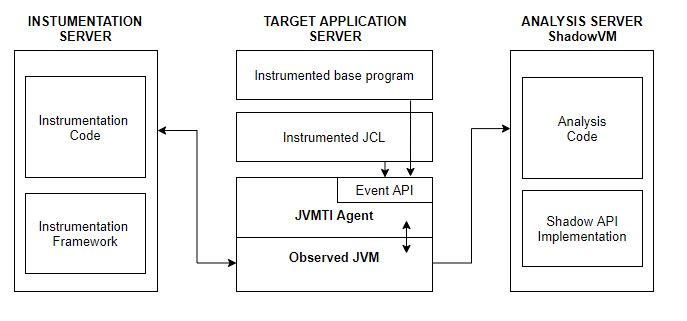
\includegraphics[scale=0.7]{Immagini/DiSL_Architecture.JPG} 
    \caption{ShadowVM architecture at a high level.}
    \label{fig:fig1}
\end{figure}

\noindent
Based on the architecture, we divide the design of our profiler into four main class modules:
\begin{itemize}
    \item \textbf{Instrumentation classes}: they are responsible for defining the actual method's instrumentation code. They ask the DiSL server to intercept specified events occurring in the target applications and inject them with DiSL code snippets. For every method of interest, instrumentation increments a specific counter, that will be then sent to the analysis server by the Local classes.
    \item \textbf{Guard classes}: they are used inside Instrumentation classes and they are responsible for the selection of the instrumentation sites for each method of interest. They also implement the DiSL Reflection API technology, exploiting reflective information of the JCL.
    \item \textbf{Local classes}: they implement the profiler inside the target application, collecting instrumented data gathered by the Instrumentation classes, in order to then send them to the analysis server.
    \item \textbf{Remote classes}: they are responsible for elaborating data collected from the profiling of the target application. They exploit ShadowVM technology, which is a separate virtual machine specifically designed for data analysis.
\end{itemize}
In the following chapters we discuss in depth the concepts just briefly introduced. 


\section{Project Structure}
Project code structure in divided following profiler modules partitioning (SCOLL, CCOLL, ELOCK, SYNCHRONIZERS, and FUTURE). Instrumentation and guard classes are further separated into main sub-topics (e.g. for the CCOLL module we divide them in BlockingQueue, ConcurrentMap, ConcurrentSkipListSet, CopyOnWriteArrayList, and CopyOnWriteArraySet). The latter division was made in order to produce code easier to read, and minimize class sizing. The final project code structure is the following:

\small
\begin{itemize}
    \item \textbf{SCOLL}:
    \begin{itemize}
        \item Instrumentation:
        \begin{itemize}
            \item \textit{Instrumentation.java}
            \item \textit{InstrumentationThread.java}
        \end{itemize}
        \item \textit{Local.java}
        \item \textit{Remote.java}
        \item \textit{Guard.java}
    \end{itemize}
    \item \textbf{CCOLL}:
    \begin{itemize}
        \item Instrumentation:
        \begin{itemize}
            \item \textit{InstrumentationBlockingQueue.java}
            \item \textit{InstrumentationConcurrentMap.java}
            \item \textit{InstrumentationConcurrentSkipListSet.java}
            \item \textit{InstrumentationCopyOnWriteArrayList.java}
            \item \textit{InstrumentationCopyOnWriteArraySet.java}
            \item \textit{InstrumentationThread.java}
        \end{itemize}
        \item \textit{Local.java}
        \item \textit{Remote.java}
        \item Guards:
        \begin{itemize}
            \item \textit{BlockingQueueGuards.java}
            \item \textit{ConcurrentMapGuards.java}
            \item \textit{ConcurrentSkipListSetGuards.java}
            \item \textit{CopyOnWriteArrayListGuards.java}
            \item \textit{CopyOnWriteArraySetGuards.java}
        \end{itemize}
    \end{itemize}
    \item \textbf{ELOCK}:
    \begin{itemize}
        \item Instrumentation:
        \begin{itemize}
            \item \textit{Instrumentation.java}
            \item \textit{InstrumentationThread.java}
        \end{itemize}
        \item \textit{Local.java}
        \item \textit{Remote.java}
        \item \textit{Guard.java}
    \end{itemize}
    \item \textbf{SYNCHRONIZERS}:
    \begin{itemize}
        \item Instrumentation:
        \begin{itemize}
            \item \textit{InstrumentationCountDownLatch.java}
            \item \textit{InstrumentationCyclicBarrier.java}
            \item \textit{InstrumentationExchanger.java}
            \item \textit{InstrumentationPhaser.java}
            \item \textit{InstrumentationSemaphore.java}
            \item \textit{InstrumentationThread.java}
        \end{itemize}
        \item \textit{Local.java}
        \item \textit{Remote.java}
        \item Guards:
        \begin{itemize}
            \item \textit{CountDownLatchGuards.java}
            \item \textit{CyclicBarrierGuards.java}
            \item \textit{ExchangerGuards.java}
            \item \textit{PhaserGuards.java}
            \item \textit{SemaphoreGuards.java}
        \end{itemize}
    \end{itemize}
    \item \textbf{FUTURE}:
    \begin{itemize}
        \item Instrumentation:
        \begin{itemize}
            \item \textit{Instrumentation.java}
            \item \textit{InstrumentationThread.java}
        \end{itemize}
        \item \textit{Local.java}
        \item \textit{Remote.java}
        \item \textit{Guard.java}
    \end{itemize}
\end{itemize}

\large
\section{Instrumentation}
In the Instrumentation part of the implementation, we represent the actual operational functions of the profiler. Using DiSL code snippets inside the instrumentation classes, we collect data on frequency of usage for every method of interest listed during the analysis phase (Chapter 3). This data will be gathered inside the Local classes, that will then redirect them to the analysis server managed by the Remote classes.

\noindent The simplest example of a code snippet that counts methods usage frequency, while taking advantage of the DiSL programming language, could be described as follows:

\vspace*{0.5cm}
\begin{minted}[fontsize=\footnotesize, linenos]{java}

@ThreadLocal
private static volatile long n_BQ_add = 0;

/*
 *  Method:
 *  boolean add(E e)
 */
@Before(marker = BodyMarker.class)
public static void beforeBQAdd(DynamicContext dc, MethodStaticContext msc) {
    if (msc.thisMethodName().equals("add") && msc.thisMethodDescriptor().equals("(Ljava/lang/Object;)Z")) {
        Object thisInstance = dc.getThis();
        if (thisInstance instanceof BlockingQueue) {
            n_BQ_add++;
        }
    }
}
\end{minted}
\vspace*{0.5cm}

\noindent
This code snippet increments a counter before every call of an \textit{add} method of the class \textit{BlockingQueue} happens. More specifically it injects inside the target application bytecode, an instruction (line 13) that increments the related counter for the \textit{add} method. Let's analyse this code line per line:

\begin{itemize}
    \item \textbf{line 2}: A specific counter for the method \textit{add} of the class \textit{BlockingQueue} is declared and initialized at zero. It is private since we want to ensure access only inside the class. It is static since we want to ensure to have the same value whatever object instance and instrumentation snippet is accessing it. And finally, volatile, so that it will be saved and accessed through memory, thereby improving thread-safety. 
    
    \item \textbf{Line 1}: This command is part of the \textit{annotations} construct offered by DiSL. It indicates that the access to the variable below (line 2) should be translated as an access to a Thread-Local variable.
    
    \item \textbf{Line 8}: It represents the instrumentation site (discussed in the background chapter). It is formed by two main entities:
    \begin{itemize}
        \item Annotation: it is made of the "@Before" part. It is an annotation that specifies where the code snippet will be inlined inside the target application: before the site specified inside the marker.
        \item Marker: it specifies that the instrumentation refers to the body of the instrumented method.
    \end{itemize}
    Together they means that the instrumentation code snippet will be injected before the first instruction of every single method body executed by the target applications.
    
    \item \textbf{Line 9}: It is the method declaration for the instrumentation snippet. It is declared static since it needs to be accessed without creating an instance of the class Instrumentation. It has two parameters:
    \begin{itemize}
        \item DynamicContext: Object that provides target application information only available to the code snippet at run-time.
        \item MethodStaticContext: Object that provides information only available to the code snippet at compile-time, about the instrumented method.
    \end{itemize}
    
    \item \textbf{Line 10}: It is the first instruction of the instrumentation code, which means that from this line to the 15Th, this instructions will be injected as bytecode inside the target applications. This particular one represents a check on the instrumented method signature. Using the \textit{MethodStaticContext} object, it queries the method name and descriptor, and then it checks if they are equals to the ones of method \textit{add}.
    
    \item \textbf{Line 11}: This instruction takes advantage of the \textit{DynamicContext} Object in order to obtain the instance of the class of the instrumented method, and then to assign it to the Object named \textit{thisInstance}.
    
    \item \textbf{Line 12}: This instruction checks if the instrumented method class obtained at line 11 is actually an instance of the class \textit{BlockingQueue}
    
    \item \textbf{Line 13}: This instruction is a simple increment of the global variable \textit{n\_BQ\_add} declared at line 2.
\end{itemize}
In summary, this instrumentation injects before the first instruction of every method executed by the target application, an equality check on its method descriptor and name with the ones of the method \textit{add}. If successful, then it checks for equality on the instance of the instrumented method class with class \textit{BlockingQueue}. If again successful, it increments the correspondent counter. Thus, If we ran this instrumentation on a target application, we would obtain the exact frequency in usage of the method \textit{add} of the \textit{BlockingQueue} class. 

\noindent
This technique is perfectly functioning, however, since we're injecting code inside every single method call of the target application, very expensive in relation to performance and overhead. To solve this problem, DiSL offers \textit{guards}. Instead of instrumenting every single method, and then checking during execution of the target application what type of method is being instrumented, with guards it is possible to carry out inspections on selected instrumentation scopes, before actually inlining code snippets. An example of guard for the code just described would look something like this:


\vspace*{0.5cm}
\begin{minted}[fontsize=\footnotesize, linenos]{java}
public class Guard{
    public final static class BlockingQueueAddMethodGuard{
    
        private BlockingQueueAddMethodGuard() {
            // Prevents instantiation
        }
    
        @GuardMethod
        public static boolean isApplicable(MethodStaticContext msc) {
            if (msc.thisMethodName().equals("add") && msc.thisMethodDescriptor().equals("(Ljava/lang/Object;)Z"))
                    return true;
            return false;
        }
    }
}
\end{minted}

\vspace*{0.5cm}

\noindent
Following DiSL criteria, guards need to be declared in separate classes, and they also need to be final and static. In order to prevent inizialitation, the constructor is set private and left empty. For the other instructions, let's analyse them line by line:


\begin{itemize}
    \item \textbf{Line 8}: This command is part of the \textit{annotations} offered by DiSL. It indicates that the method below represent a guard.
    
    \item \textbf{Line 9-13}: It is the actual guard method implementation. The content is almost the same compared with the content of the guard-less instrumentation code snippet. However, the dynamic check on the class is not present and the operations computed after the checks change: the method returns a boolean variable, instead of incrementing the target method variable.
\end{itemize}

\noindent
With this guard, it is possible to remove the static instrumentation site checks from the instrumentation completely. However, the dynamic checks would still be necessary inside the instrumentation, achieving a code that would look like the following:


\vspace*{0.5cm}
\begin{minted}[fontsize=\footnotesize, linenos]{java}

@ThreadLocal
private static volatile long n_BQ_add = 0;

/*
 *  Method:
 *  boolean add(E e)
 */
@Before(marker = BodyMarker.class, guard = Guard.BlockingQueueAddMethodGuard.class)
public static void beforeBQAdd(DynamicContext dc) {
    Object thisInstance = dc.getThis();
    if (thisInstance instanceof BlockingQueue)
        n_BQ_add++;
}
\end{minted}

\vspace*{0.5cm}

\noindent
Modifications can be found at lines:
\begin{itemize}
    \item \textbf{line 8}: Instrumentation site have been now augmented with the guard check, that simply indicates the path where to find the guard.
    
    \item \textbf{Line 10-12}: All static checks have been removed, leaving the increment and the dynamic checks as the only instructions necessary.
\end{itemize}

\noindent
With this method we can achieve two benefits:
\begin{enumerate}
    \item \textbf{Cleaner code}: After removing static checks, it is now easier to focus on the actual task that we want to achieve with the instrumentation.
    
    \item \textbf{Performance boost}: All static checks are now done before injecting the code inside the target application, improving performance slightly.
\end{enumerate}

\noindent
Further explanations on specific guard implementation for this profiler will be discussed in the following chapter. It was however necessary to introduce this concept to fully understand following Instrumentation code.

\subsection{Nested Methods}
The example just provided does not take in consideration the concept of nested methods, already discussed in the analysis chapter (chapter 3). For "nested methods" we refer to all the methods of interest that are called inside the implementation of other methods of interest. When profiling target applications with the instrumentation code just described in the previous example, we would be counting all the methods of interest. However, profiling would be automatically extended to the nested methods as well. For example, the \textit{add} method of class \textit{CopyOnWriteArraySet} calls -inside its implementation- the \textit{addIfAbsent} method, which is also part of the methods of interest list:

\begin{minted}[linenos]{java}
public boolean add(E e) {
    return al.addIfAbsent(e);
}
\end{minted}

\noindent
With the instrumentation code example previously provided, we would be increasing frequency counters for both methods. This is not necessarily an error, since the \textit{addIfAbsent} method is actually being executed. However, with this profiler, we want to gather information about active method usage only. Thereby, we had to figure out a way to avoid instrumentation of nested methods. The approach we came up with is described in the following example:



\vspace*{0.5cm}
\begin{minted}[fontsize=\footnotesize, linenos]{java}

/* Global Counter */
@ThreadLocal
private static volatile long global_counter = 0;

/* Method Specific Counter */
@ThreadLocal
private static volatile long n_BQ_add = 0;

/*
 *  Method:
 *  boolean add(E e)
 */

@Before(marker = BodyMarker.class, guard = BlockingQueueGuards.BlockingQueueAddGuardFL.class)
public static void beforeBQAddMethod() {
    Object thisInstance = dc.getThis();
    if (thisInstance instanceof BlockingQueue)
    global_counter++;
}

@After(marker = BodyMarker.class, guard = BlockingQueueGuards.BlockingQueueAddGuardFL.class)
public static void afterBQAddMethod() {
    Object thisInstance = dc.getThis();
    if (thisInstance instanceof BlockingQueue)
    global_counter--;
    if (global_counter == 0)
        n_BQ_add++;
}
\end{minted}
\vspace*{0.5cm}

Compared with the previous basic example, additions to the code can be summarized as:
\begin{itemize}
    \item \textbf{Global Counter}: We added a global counter shared between all instrumentation snippets. It is declared and instantiated in the same exact way as the method specific counter, already explained in the previous example. [Lines 1-3]
    \item \textbf{Before Snippet Behaviour}: we chanced the behaviours of the snippet marked with the \textit{@Before} annotation. Instead on incrementing the specific method counter, we now increment the global one. [Line 16]
    \item \textbf{@After Annotation}: After the \textit{@Before} annotation, we also added an instrumentation snippet marked with an \textit{@After} annotation. This means that the code specified inside this snippet will be injected after the last instruction of the target method. Here, we decrease the global counter by 1, then check if the latter is equals to 0, in which case we increment the specific method counter. [Lines 19-24]
\end{itemize}

\noindent
With this approach, all the \textit{@Before} snippets are executed before the ones marked with the \textit{@After} annotation. So, when accessing the first method, ergo the method of interest, if no nested methods are present, then simply the global counter is decremented, and the specific method counter increased by one. However, if any nested methods are present, global counter is again incremented by one (or more, depending on the number of nested methods), reaching value equals to 2 (or more). But then, when accessing the after snippet, the global counter is decremented, reaching value equals to 1, and the checks on it then do not pass, leaving the specific nested method counter still equals to zero. Only the counter for the method of interest is incremented, after global counter reaches value 0. So, taking in consideration the example of instrumenting method \textit{add} of class \textit{CopyOnWriteArraySet} we generate the following computation:
\begin{enumerate}
    \item The before snippet for method \textit{add} is executed:
    \begin{itemize}
        \item global\_counter = 1
        \item add\_counter = 0
        \item addIfAbsent\_counter = 0
    \end{itemize}
    \item The before snippet for nested method \textit{addIfAbsent} is executed:
    \begin{itemize}
        \item global\_counter = 2
        \item add\_counter = 0
        \item addIfAbsent\_counter = 0
    \end{itemize}
    \item The after snippet for nested method \textit{addIfAbsent} is executed:
    \begin{itemize}
        \item global\_counter = 1
        \item add\_counter = 0
        \item addIfAbsent\_counter = 0
    \end{itemize}
    \item The after snippet for nested method \textit{add} is executed:
    \begin{itemize}
        \item global\_counter = 0
        \item add\_counter = 1
        \item addIfAbsent\_counter = 0
    \end{itemize}
\end{enumerate}
With this process is, therefore, possible to avoid counting of nested methods.

\subsection{Thread Instrumentation}
The final goal of this thesis dissertation is to present a profiler that can be run onto benchmarks, to analyse their method usage frequencies of concurrent libraries of the JCL. Benchmarks usually run through iterations. Therefore, we wanted to build a profiler that could also manage them. In order to do so, we instrument Thread execution. Further explanation will be provided in the following chapters (4.4 Local). However, for now, it is useful to know that in every profiler module, there is a class named \textit{InstrumentationThread.java}, which task is to register the start and the termination of a Thread. The implementation code is the  following:

\vspace*{0.5cm}
\begin{minted}[fontsize=\footnotesize, linenos]{java}
@Before(marker = BodyMarker.class, guard = GuardsPreprocessing.ThreadRunGuardFL.class)
public static void beforeThreadRunFL() {
    Local.registerThreadExecutionStart(Thread.currentThread());
}


@After(marker = BodyMarker.class, guard = GuardsPreprocessing.ThreadRunGuardFL.class)
public static void afterThreadRunFL() {
    Local.registerThreadExecutionEnd(Thread.currentThread());
}
\end{minted}
\vspace*{0.5cm}

\noindent
It uses guards that exploits DiSL Reflection API to check for Thread execution. When the \textit{run()} method is called, a registration of a started execution is stored inside the \textit{Local} class, besides the instance reference of the currently executed thread object. The same happens when it ends.

\section{Guards}
In order to understand guards implementation, it is firstly necessary to expand on the concept of DiSL Reflection API, already introduced in the background chapter (chapter 2).

\subsection{DiSL Reflection API}
According to the explanations of instrumentation code provided in the previous chapter (chapter 3), we are now able to instrument all methods of interest, one by one. However, most of them are inherited from parent classes, or are themselves methods of super classes to be inherited. For example, let's follow the one provided in the previous chapter (chapter 3), where we presented the code instrumentation for method \textit{add} of interface \textit{BlockingQueue}. This method is inherited in the following sub-classes and sub-interfaces: 
\begin{itemize}
    \item BlockingDeque<E>
    \item TransferQueue<E>
    \item ArrayBlockingQueue<E>
    \item DelayQueue<E extends Delayed>
    \item LinkedBlockingQueue<E>
    \item PriorityBlockingQueue<E>
    \item SynchronousQueue<E>
    \item LinkedBlockingDeque<E>
    \item LinkedTransferQueue<E>
\end{itemize}
In order to create code instrumentation for the \textit{add} method of all them, we would have to implement code snippets for every single class. Thus, creating apparently useless repetition in the implementation code, that is however necessary in order to build a correctly functioning profiler. Another way of instrumenting could be done as follows:

\vspace*{0.5cm}
\begin{minted}[fontsize=\footnotesize, linenos]{java}
@Before(marker = BodyMarker.class)
public static void beforeBQAddFail(DynamicContext dc, MethodStaticContext msc) {
    if (msc.thisMethodName().equals("add") && msc.thisMethodDescriptor().equals("(Ljava/lang/Object;)Z")) {
        Object thisInstance = dc.getThis();
        if (thisInstance instanceof BlockingQueue) {
            global_counter++;
        }
    }
}

@After(marker = BodyMarker.class)
public static void afterBQAddFail(DynamicContext dc, MethodStaticContext msc) {
    if (msc.thisMethodName().equals("add") && msc.thisMethodDescriptor().equals("(Ljava/lang/Object;)Z")) {
        Object thisInstance = dc.getThis();
        if (thisInstance instanceof BlockingQueue) {
            global_counter--;
            if (global_counter == 0)
                n_BQ_add++;
        }
    }
}
\end{minted}
\vspace*{0.5cm}

\noindent
As already seen in the previous chapter (chapter 3), we could place the static checks inside a separate guard (lines 3 and 13) and produce cleaner and better performing code. Dynamic checks (lines 4, 5, 14, 15), however, would still be left inside instrumentation code. This represents a huge problem, since they are very expensive in terms of performance, and, when injected inside the target application, raise the overhead quite a lot.

\noindent
\textbf{DiSL Reflection API} solves this problem, providing reflective information for classes of the JCL. It works by preprocessing the entire class hierarchy of the JCL, before running the JVM. These information are stored and made accessible through \textit{ReflectionStaticContext} objects as static contexts, thus accessible by guards. This operation is quite expensive in terms of execution time, however the perks are multiple:
\begin{itemize}
    \item \textbf{Better profiling performance}: Since preprocessing of the JCL hierarchy is performed before the actual profiling analysis starts, the latter will not be affected however long it will take to conclude gathering of reflective information. Rather, removing dynamic checks improves profiling performance considerably.
    \item \textbf{Necessity to be run only once}: Once the JVM has been preprocessed, reflective information are stored indefinitely, and -unless we actively remove them- the profiler will be able to access them, without ever having to run the analysis again.
    \item \textbf{Cleaner Instrumentation Code}: Since reflective information can now be accessed through guards, instrumentation code snippets can be used exclusively to implement operational behaviours, leaving instrumentation site checks out, improving separation of concerns.
\end{itemize}
Therefore, even though gathering of reflective information will take quite a lot of time, it will only benefits the profiler performances and code structure. 

\vspace*{0.5cm}
\noindent
Let's now see how the final implementation of the instrumentation code of the method \textit{add} of interface \textit{BlockinQueue} -and all of its subclasses and sub interfaces- looks like using DiSL Reflection API:


\vspace*{0.5cm}
\begin{minted}[fontsize=\footnotesize, linenos]{java}
/* Global Counter */
@ThreadLocal
private static volatile long global_counter = 0;

/* Method Specific Counter */
@ThreadLocal
private static volatile long n_BQ_add = 0;

/*
 *  Method:
 *  boolean add(E e)
 */

@Before(marker = BodyMarker.class, guard = BlockingQueueGuards.BlockingQueueAddGuardFL.class)
public static void beforeBQAddMethod() {
    global_counter++;
}

@After(marker = BodyMarker.class, guard = BlockingQueueGuards.BlockingQueueAddGuardFL.class)
public static void afterBQAddMethod() {
    global_counter--;
    if (global_counter == 0)
        n_BQ_add++;
}
\end{minted}
\vspace*{0.5cm}
Instrumentation code snippets implements only the profiler operation logic (lines 16, 21, 22, and 23) leaving the instrumentation sites checks to the guards.

\subsection{Preprocessor Set-Up}
In order to set-up preprocessing of the JCL with the methods and classes of interest, several steps are necessary:
\begin{enumerate}
    \item \textbf{White-Lists}: first of all, we need to provide the profiler with the list of methods of interest. In order to do so, we created, in a folder called \textit{preprocesser}, another folder called \textit{input}, where we inserted standard text documents (\textit{.txt} format), every one of them containing the full method name of the corresponding method of interest. These files are called \textit{white-lists}, and they are used during preprosessing to match all the classes that are subtypes of the specified class with the specified method.
    \vspace{0.5cm}
    \begin{figure}[h]
        \centering
        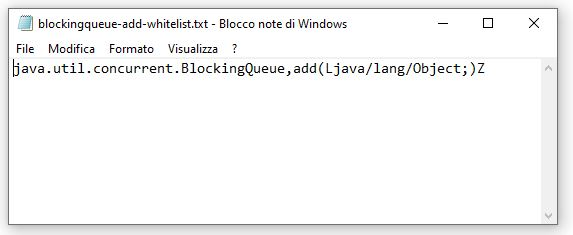
\includegraphics[scale=0.7]{Immagini/whitelist.JPG} 
        \caption{White-List for method \textit{add} of class \textit{BlockingQueue}.}
        \label{fig:fig1}
    \end{figure}
    \vspace{0.5cm}
    \newline In the example in figure 4.1, we represent the white-list for method \textit{add} of class \textit{BlockingQueue}. Therefore, every subclass of \textit{BlockingQueue} of package \textit{java.util.concurrent}, implementing a method name \textit{add}, receiving in input an \textit{Object} and returning a \textit{boolean}, will be added to the analysis.
    \newline Every white-list corresponds to a method usage frequency counter produced by the profiler after the analysis is completed. For counters made of multiple methods, the corresponding white-list needs to be written specifying every single method. So, for example, figure 4.2 represents the white-list for the methods \textit{V remove(Object key)} and \textit{boolean remove(Object key, Object value)} of class \textit{SynchronizedMap} that we decided to merge in a single counter. The preprocessor will match every subtype of class \textit{SynchronizedMap} that implements both methods.
    \vspace{0.5cm}
    \begin{figure}[h]
        \centering
        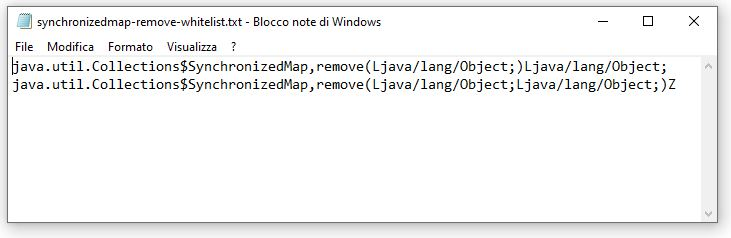
\includegraphics[scale=0.7]{Immagini/whitelist-double.JPG} 
        \caption{White-List for methods \textit{boolean remove(Object key, Object value)} and \textit{V remove(Object key)} of class \textit{SynchronizedMap}.}
        \label{fig:fig1}
    \end{figure}
    \vspace{0.5cm}
    \item \textbf{Black-Lists}: Opposed to the white-lists, there are the \textit{black-lists}. For every counter, it is possible to specify inside separate standard text documents lists of methods not to be profiled, representing an exception on the ones inserted inside the white-lists. In this case we didn't need any of these, so we left the documents blank.
    \item \textbf{Preprosessor script modification}: For every inserted white and black list, the preprosessor scripts need to be updated with the new information. In particular the bash file \textit{preprocess.sh} which is responsible for collecting information inserted inside the white and black lists. It then forwards them to the \textit{do\_preprocess.sh} script. In the latter, the actual preprocessing operations are described. We will not explain in detail the scripting operations, since their not part of the project workload developed for this thesis dissertation. However, we deem useful to mention them for contextual reference.
\end{enumerate}

\subsection{Preprocessing Results}
When starting the profiler, the preprocessor will run automatically (if not already done previously). The output of the preprocessor will be the list of methods of interest generated from the ones specified in the white-lists file. Following the example described in figure 4.2, after running the will be generated. The content of this file is described in figure 4.3, and it represent the full name for both \textit{remove} methods specified in the white-list file, for class \textit{SynchronizedMap} and inheriting classes. Specifically:
\begin{itemize}
    \item V remove(Object key) for class SynchronizedMap
    \item boolean remove(Object key, Object value) for class SynchronizedMap
    \item V remove(Object key) for class SynchronizedNavigableMap
    \item boolean remove(Object key, Object value) for class SynchronizedNavigableMap
    \item V remove(Object key) for class SynchronizedSortedMap
    \item boolean remove(Object key, Object value) for class SynchronizedSortedMap
\end{itemize}

\vspace{0.5cm}
\begin{figure}[h]
    \centering
    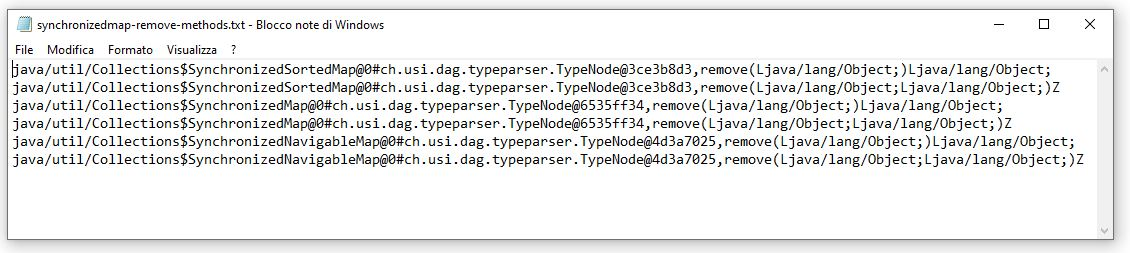
\includegraphics[scale=0.45]{Immagini/outputmethods.JPG} 
    \caption{Methods of interest resulting as preprocessor output for methods \textit{boolean remove(Object key, Object value)} and \textit{V remove(Object key)} of class \textit{SynchronizedMap}.}
    \label{fig:fig1}
\end{figure}
\vspace{0.5cm}


\newline
\noindent
Every time one of these method will be used during profiling by the target application, the corresponding instrumentation will be triggered, increasing the respective method usage frequency counter.

\subsection{Guards Implementation}
Guards implementation that exploits DiSL Reflection API it's pretty straight forward. Let's analyse the corresponding code for method \textit{add} of class \textit{BlockingQueue}:

\vspace*{0.5cm}
\begin{minted}[fontsize=\scriptsize, linenos]{java}
private static final String BLOCKINGQUEUE_ADD_PREPROCESS_FILE_PROPERTY_NAME = "dag.preprocess.blockinqueueaddfile";
private static final String BLOCKINGQUEUE_ADD_PREPROCESS_FILE_DEFAULT= "input/blockingqueue-add-typegraph.ser";

private static PreprocessingHelper BlockingQueue_AddHelper = new PreprocessingHelper(
                                                            Properties.stringFromPropertyOrDefault(
                                                                    BLOCKINGQUEUE_ADD_PREPROCESS_FILE_PROPERTY_NAME,
                                                                    BLOCKINGQUEUE_ADD_PREPROCESS_FILE_DEFAULT));


private final static class BlockingQueueAddClassGuard {

    @GuardMethod
    public static boolean isApplicable(ReflectionStaticContext rsc) {
        return BlockingQueue_AddHelper.shallClassBeInstrumented(rsc.thisClass());
    }
}

private final static class BlockingQueueAddMethodGuard {

    @GuardMethod
    public static boolean isApplicable(MethodStaticContext msc, ReflectionStaticContext rsc) {
        return BlockingQueue_AddHelper.shallMethodBeInstrumented(rsc.thisClass(), msc.thisMethodName() +
                                                                      msc.thisMethodDescriptor());
    }
}

public final static class BlockingQueueAddGuardFL {

    private BlockingQueueAddGuardFL() { /* Prevent instantiation */ }

    @GuardMethod
    public static boolean isApplicable(final GuardContext gc, final MethodStaticContext msc, ReflectionStaticContext rsc) {

        boolean result = false;

        if (BlockingQueue_AddHelper.isTargetMethod(msc.thisMethodName() + msc.thisMethodDescriptor())) {
            result = gc.invoke(BlockingQueueAddClassGuard.class) && gc.invoke(BlockingQueueAddMethodGuard.class);

        }

        return result;

    }
}
\end{minted}
\vspace*{0.5cm}
 
 In the example above guard structuring is set up as follows:
\begin{itemize}
    \item \textbf{Lines 1-2}: The files generated during the preprocessing phase for the \textit{add} method of class \textit{BlockingQueue} are loaded and saved inside this two global string variables.
    \item \textbf{Line 4}: The string variables at line 1 and 2 are now used to create the \textit{PreprocessingHelper} Object. This construct uses the information contained inside of them, in order to build the JCL hierarchy of the classes of interest in example.
    \item \textbf{Lines 10-16}: This first guard checks if the class of the method that is being instrumented is an instance of \textit{BlockingQueue}, or a subtype of it. It uses the information contained in \textit{ReflectionStaticContext} object, and it compares them with the ones inside the \textit{BlockingQueue\_AddHelper} object.
    \item \textbf{Lines 18-25}: This second guard checks if the the method that is being instrumented is method \textit{add} of class \textit{BlockingQueue} (or a subtype of it), thus the method of interest. It uses the information contained in \textit{ReflectionStaticContext} object, and in the \textit{MethodStaticContextObject} and it compares them with the ones inside the \textit{BlockingQueue\_AddHelper} object.
    \item \textbf{Lines 27-44}: This third, and last, guard, is the only one called by the Instrumentation, thereby the only declared public. It calls both guards just described above, and in case they both return a true value, it reports to the Instrumentation that the current method is a method of interest.
\end{itemize}
The same implementation is repeated for every single method that takes advantage of the DiSL Reflection API.



\subsection{Guards Implementation without DiSL Reflection API}
We just described how to implement guards for methods of interest of which profiling exploits the DiSL Reflection API. However, this technology is not useful for every method of interest. In fact, there are methods that cannot be overridden by other classes: static methods. They are not polymorphic, thus statically linked at compile time. This makes usage of reflective information useless, and for this particular reason, also guards implementation changes. Let's analyse an example for static method \textit{synchronizedCollection} of class Collections:


\vspace*{0.5cm}
\begin{minted}[fontsize=\footnotesize, linenos]{java}
public final static class CollectionsSynchronizedCollectionGuard {

    private final static String targetMethod = "java/util/Collections.synchronizedCollection(
                                                      Ljava/util/Collection;)Ljava/util/Collection;";


    private CollectionsSynchronizedCollectionGuard() {
        // Prevents instantiation
    }

    @GuardMethod
    public static boolean isApplicable(InvocationStaticContext isc) {
        return isc.getUniqueInternalName().equals(targetMethod);
    }
}
\end{minted}
\vspace*{0.5cm}
Without DiSL Reflection API, implementation is a lot simpler. At line 13, it uses the \textit{InvocationStaticContext} object to equality check on the instrumented method, compared with the method of interest specified at line 3.


\section{Local}
With the instrumentation classes we are able to identify methods of interest, increase corresponding counters, and catch thread execution. Local classes have the duty to collect these data and send them to the analysis server. To achieve this task, they implement a sort of profiler, that is executed inside the target application JVM. It gathers information profiled by the instrumentation classes, and dispatch them to the detached analysis JVM. Communication through JVMs is achieve utilizing the \textit{REDispatch} class. 

\subsection{REDispatch}
REDispatch is a DiSL API used inside Local classes, that provides to the clients of the Shadow VM (i.e. the analysis server), an interface to invoke and register remote analysis methods. Usage of this class should follow these steps:
\begin{itemize}
    \item \textbf{Method registering}: using the method \textit{registerMethod(String)}, and providing in input a fully qualified method name, we register each remote analysis method on the analysis server.
    \vspace*{0.5cm}
    \begin{minted}[fontsize=\footnotesize, linenos]{java}
private static final String METHOD_PREFIX = "ch.usi.dag.concurrency.benchmark.synchronizers.Remote.";
private static final short registerThreadStartID = REDispatch.registerMethod(METHOD_PREFIX +
                                                                        "registerThreadStart");
\end{minted}
\vspace*{0.5cm}
    In this example we register thread start registration method, providing the fully qualified method name made of: classfile path of the Remote class and method name.
    \item \textbf{Method invocation}: using the method \textit{analysisStart(short)} we then specify which method will need to be called inside the ShadowVM when data will be received.
    \vspace*{0.5cm}
    \begin{minted}[fontsize=\footnotesize, linenos]{java}
REDispatch.analysisStart(registerThreadStartID);
\end{minted}
\vspace*{0.5cm}
    In this example we specify invocation for the thread start registration method just registered.
    \item \textbf{Data dispatch}: using various methods, we send the necessary data to the ShadowVM.
    \vspace*{0.5cm}
    \begin{minted}[fontsize=\footnotesize, linenos]{java}
REDispatch.sendObjectPlusData(thread.getName());
REDispatch.sendInt(System.identityHashCode(thread));
REDispatch.sendLong(System.nanoTime());
\end{minted}
\vspace*{0.5cm}
    In this example we send profiled data for thread initiation: thread name, thread hashcode, and thread initiation time. 
    \item \textbf{Method Invocation End}: To end invocation sequence, after the necessary data has been sent to the analysis server, it is necessary to call the method \textit{analysisEnd()}.
    \vspace*{0.5cm}
    \begin{minted}[fontsize=\footnotesize, linenos]{java}
REDispatch.analysisEnd();
\end{minted}
\vspace*{0.5cm}
\end{itemize}


\subsection{Implementation}
Local class implementation is structured as follows:

\begin{itemize}
    \item \textbf{Instrumentation fields}: It is a private static array of Strings, containing all the frequency counters profiled by the Instrumentation. For example, in the Local class for SYNCHRONIZERS profiler module we have:
    
\vspace*{0.25cm}
    \begin{minted}[fontsize=\footnotesize, linenos]{java}
    private static String[] __instrumentationFields = {
            "n_Semaphore_acquire",
            "n_Semaphore_drainPermits",
            "n_Semaphore_release",
            "n_Semaphore_tryAcquire",
            "n_CTL_await",
            "n_CTL_countDown",
            "n_CB_await",
            "n_CB_reset",
            "n_Phaser_arrive",
            "n_Phaser_arriveAndAwaitAdvance",
            "n_Phaser_arriveAndDeregister",
            "n_Phaser_awaitAdvance",
            "n_Phaser_bulkRegister",
            "n_Phaser_forceTermination",
            "n_Phaser_register",
            "n_Exchanger_exchange"
    };
    \end{minted}
    \vspace*{0.25cm}
    which are exactly the names given to all frequency counters specified in this profiler. They will also represent the data fields provided as output of the profiler analysis.
    \item \textbf{Active threads list}: It is a ConcurrentSkipListSet (i.e. ordered list that ensures thread-safety) of the active threads.
    \vspace*{0.25cm}
    \begin{minted}[fontsize=\footnotesize, linenos]{java}
private static final ConcurrentSkipListSet<Thread> __activeThreads;
        \end{minted}
        \vspace*{0.25cm}
    When a thread starts, it is inserted inside this set. When it ends, it is then removed.
    
    \item \textbf{Thread execution management}: Thread execution data collection and dispatch is achieved through various steps:
    \begin{enumerate}
         \item \textbf{Thread execution and metrics registration}: thread start (line 1), thread end (line 3), and metrics (line 5) registration methods are registered inside the ShadowVM:
         
        \vspace*{0.25cm}
        \begin{minted}[fontsize=\footnotesize, linenos]{java}
private static final short registerThreadStartID = REDispatch.registerMethod(METHOD_PREFIX 
                                                                        + "registerThreadStart");
private static final short registerThreadEndID = REDispatch.registerMethod(METHOD_PREFIX 
                                                                        + "registerThreadEnd");
private static final short registerMetricID = REDispatch.registerMethod(METHOD_PREFIX 
                                                                            + "registerMetric");
    \end{minted}
        \vspace*{0.25cm}
        \item \textbf{Thread start registration and data dispatch}: The starting thread is added to the active threads list (line 2). Then, through REDispatch, the necessary thread data is sent to the ShadowVM (line 3, and lines 6-14):
        \vspace*{0.25cm}
        \begin{minted}[fontsize=\footnotesize, linenos]{java}
public static synchronized void  registerThreadExecutionStart(Thread thread) {
    __activeThreads.add(thread);
    __registerThreadStart(thread);
}

private static void __registerThreadStart(Thread thread) {
    REDispatch.analysisStart(registerThreadStartID, GLOBAL_ORDER);
    
    REDispatch.sendObjectPlusData(thread.getName());
    REDispatch.sendInt(System.identityHashCode(thread));
    REDispatch.sendLong(System.nanoTime());

    REDispatch.analysisEnd();
}
    \end{minted}
    \vspace*{0.25cm}
        \item \textbf{Thread end registration  and data dispatch}: Instrumentation fields -and corresponding metrics collected during thread execution- are registered and sent to the analysis server (line 3 and lines 9-32). Then, the ending thread is removed from the list of active threads (line 4). Finally, Thread execution termination is registered and corresponding data is sent through REDispatch (line 6, and lines 34-42):
        \vspace*{0.25cm}
        \begin{minted}[fontsize=\footnotesize, linenos]{java}
public static synchronized void registerThreadExecutionEnd(Thread thread) {
    synchronized(Local.class) {
        __registerInstrumentationFields(thread);
        __activeThreads.remove(thread);
    }
    __registerThreadEnd(thread);
}

private static void __registerInstrumentationFields(Thread thread) {
    for (String fieldName : __instrumentationFields ) {
        try {
            Field field = __threadClass.getDeclaredField(fieldName);
            long value = field.getLong(thread);
            __registerMetric(thread, fieldName, value);
        } catch (Exception e) {
            System.err.println("Error while accessing instrumentation field " + fieldName);
            e.printStackTrace();
        }
    }
}

private static void __registerMetric(Thread thread, String fieldName, long value) {

    REDispatch.analysisStart(registerMetricID, GLOBAL_ORDER);

    REDispatch.sendInt(System.identityHashCode(thread));
    REDispatch.sendObjectPlusData(fieldName);
    REDispatch.sendLong(value);

    REDispatch.analysisEnd();

}

private static void __registerThreadEnd(Thread thread) {
    REDispatch.analysisStart(registerThreadEndID, GLOBAL_ORDER);

    REDispatch.sendObjectPlusData(thread.getName());
    REDispatch.sendInt(System.identityHashCode(thread));
    REDispatch.sendLong(System.nanoTime());

    REDispatch.analysisEnd();
}
    \end{minted}
    \vspace*{0.25cm}
        
    \end{enumerate}
    
    \item \textbf{Benchmark iterations management}: Benchmark iterations data collection and dispatch is achieved through various steps:
    \begin{enumerate}
        \item \textbf{Benchmark iteration registration}: first of all, we register inside the analysis server the method to be called when benchmark iteration data will be sent to it:
        
        \vspace*{0.25cm}
        \begin{minted}[fontsize=\footnotesize, linenos]{java}
private static final short registerIterationID = REDispatch.registerMethod(METHOD_PREFIX 
                                                                + "registerIterationStart");
    \end{minted}
    \vspace*{0.25cm}
    \item \textbf{Benchmark iteration start}: before a new benchmark iteration starts, we firstly add the current thread to the active threads list (line 2). Then, for every thread inside of it -which are thread not yet terminated-, we send to the analysis server all the collected metrics (lines 4-6). Finally, we report the the Shadow VM that a new benchmark iteration is starting (line 8, and line 11-15):
    \vspace*{0.25cm}
        \begin{minted}[fontsize=\footnotesize, linenos]{java}
public static synchronized void beforeIteration() {
    __activeThreads.add(Thread.currentThread());

    for (Thread thread: __activeThreads ) {
        __registerInstrumentationFields(thread);
    }

    __registerIterationNumber(Common.iteration);
}

private static void __registerIterationNumber(int iteration) {
    REDispatch.analysisStart(registerIterationID, GLOBAL_ORDER);
    REDispatch.sendInt(iteration);
    REDispatch.analysisEnd();
}
    \end{minted}
    \vspace*{0.25cm}
    \item \textbf{Benchmark iteration end}: when a benchmark iteration comes to an end, we repeat the same process: adding the current thread to the active threads list, then sending to the analysis server, for every thread still active, all the collected metrics, finally, reporting to the the Shadow VM that the running benchmark iteration is terminating.
    \end{enumerate}
\end{itemize}


\section{Remote}
In the Remote classes we receive data collected and sent by the Local classes. They run onto a seperate JVM, the Shadow VM, which represents the analysis server of the profiler. Here, gathered information are organized and printed inside the two following matrix files:
\begin{itemize}
    \item \textit{metrics.csv}: this file contains the information collected during the analysis, regarding methods usage frequency. Each frequency counter has its corresponding data, divided by benchmark iteration. Iterations represented by positive numbers refers to findings collected during the execution of an iteration, while negatives represents data collected between iterations.
    
    \vspace{0.5cm}
\begin{figure}[h]
    \centering
    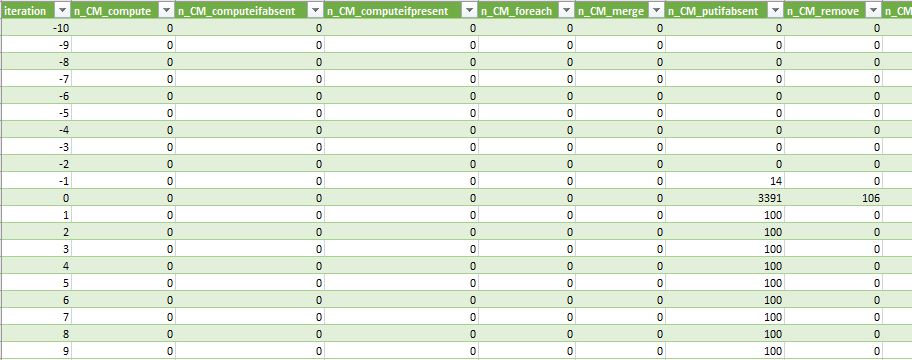
\includegraphics[scale=0.6]{Immagini/metricscsv.JPG} 
    \caption{Example of file metrics.csv for CCOLL profiler module.}
    \label{fig:fig1}
\end{figure}
\vspace{0.5cm}
    \item \textit{thread.csv}: this files contains the timestamps in nanoseconds for each executed thread during the analysis. The file is divided in:
    \begin{itemize}
        \item Name of executed thread.
        \item ID of executed thread.
        \item Benchmark iteration number where the executed thread started.
        \item Benchmark iteration number where the executed thread ended.
        \item Timestamp for when the executed thread started.
        \item Timestamp for when the executed thread ended.
    \end{itemize}
    \vspace{0.5cm}
\begin{figure}[h]
    \centering
    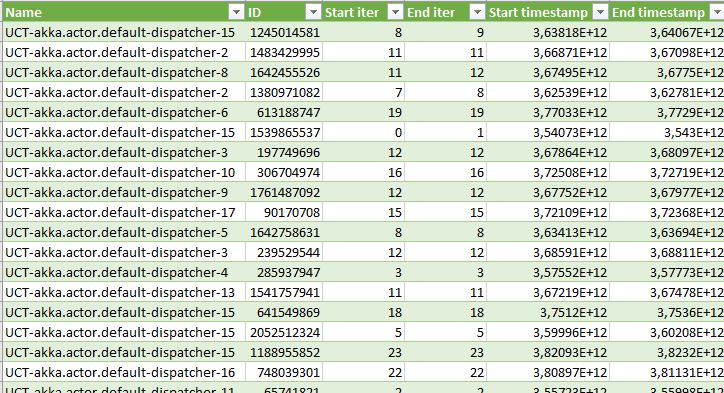
\includegraphics[scale=0.6]{Immagini/threadcsv.JPG} 
    \caption{Example of file thread.csv profiler module.}
    \label{fig:fig1}
\end{figure}
\end{itemize}

\noindent
This class extend the abstract class \textit{RemoteAnalysis} [DRAFT: SHADOW OBJECTS]

\subsection{Code Structure}
Implementation structure is corresponding to the final products of this class execution: creating the matrices for methods usage frequency and threads execution. Let's firstly analyse the latter:

\subsubsection{Thread Execution}
Thread profiling data is organized inside a ConcurrentHashMap (i.e. a key-value map that ensures thread-safety) where the threads ID are used as keys, and the remaining information as values, encapsulated in an object called \textit{ThreadProfile}:

    \vspace*{0.25cm}
        \begin{minted}[fontsize=\footnotesize, linenos]{java}

private ConcurrentHashMap<Integer, ThreadProfile> __threadProfileMap;
        
private static class ThreadProfile  {
    String threadName = null;
    int threadID = -1;
    int startIter = Integer.MAX_VALUE;
    int endIter = Integer.MAX_VALUE;
    long startTimestamp = -1;
    long endTimestamp = -1;

    public ThreadProfile(String name, int id ) {
        threadName = name;
        threadID = id;
    }

    public static String[] getHeader() {
        String[] header = {
                "Name",
                "ID",
                "Start iter",
                "End iter",
                "Start timestamp",
                "End timestamp"
        };
        return header;
    }

    public String[] toStringArray() {
        String[] strArray = {
                threadName,
                Integer.toString(threadID),
                Integer.toString(startIter),
                Integer.toString(endIter),
                Long.toString(startTimestamp),
                Long.toString(endTimestamp),
        };
        return strArray;
    }
}
    \end{minted}
    \vspace*{0.25cm}
    
    \noindent
    Implementation of the methods registered inside Local classes, are here provided. Method \textit{registerThreadStart} adds to the\textit{ \_\_threadProfileMap} object a new instance of \textit{ThreadProfile}, filling it with current thread name, id, benchmark iteration and starting timestamp information provided by the REDispatch API executed from the Local classes (lines 1-8). The same is then repeated in the \textit{registerThreadEnd} method for ending threads (lines 10-17).
    
    \vspace*{0.25cm}
        \begin{minted}[fontsize=\footnotesize, linenos]{java}
public void registerThreadStart(final ShadowString name, final int id, final long timestamp) {

    final ThreadProfile prof = __threadProfileMap.computeIfAbsent(id, (t) -> new ThreadProfile(name.toString(), id));

    prof.startTimestamp = timestamp;
    prof.startIter = __currentIteration;

}

public void registerThreadEnd(final ShadowString name, final int id, final long timestamp) {

    final ThreadProfile prof = __threadProfileMap.computeIfAbsent(id, (t) -> new ThreadProfile(name.toString(), id));

    prof.endTimestamp = timestamp;
    prof.endIter = __currentIteration;

}
    \end{minted}
    \vspace*{0.25cm}
    
\subsubsection{Methods Usage Frequency}
 Methods usage frequency profiling is organized inside a ConcurrentHashMap where the executing threads ID are used as keys. As values, it is utilized another ConcurrentHashMap, with the number of the current executed iteration used as keys, and the methods usage frequency information -encapsulated in an object called \textit{MetricProfile}- as values.
    \vspace*{0.25cm}
        \begin{minted}[fontsize=\scriptsize, linenos]{java}
private ConcurrentHashMap<Integer, ConcurrentHashMap<Integer, MetricProfile>> __threadToMetricProfileMap;

private static class MetricProfile  {
    int iteration;
    long n_Semaphore_acquire = 0;
    long n_Semaphore_drainPermits = 0;
    long n_Semaphore_release = 0;
    long n_Semaphore_tryAcquire = 0;
    long n_CTL_await = 0;
    long n_CTL_countDown = 0;
    long n_CB_await = 0;
    long n_CB_reset = 0;
    long n_Phaser_arrive = 0;
    long n_Phaser_arriveAndAwaitAdvance = 0;
    long n_Phaser_arriveAndDeregister = 0;
    long n_Phaser_awaitAdvance = 0;
    long n_Phaser_bulkRegister = 0;
    long n_Phaser_forceTermination = 0;
    long n_Phaser_register = 0;
    long n_Exchanger_exchange = 0;

    public MetricProfile(int iter) {
        super();
        iteration = iter;
    }

    public static MetricProfile difference(int newIter, MetricProfile profile1, MetricProfile profile2) {
        MetricProfile result = new MetricProfile(newIter);

        for (Field field : MetricProfile.class.getDeclaredFields()) {
            if (field.getName().equals("iteration")) {
                continue;
            }
            try {
                long fieldProfile1 = field.getLong(profile1);
                long fieldProfile2 = field.getLong(profile2);
                field.setLong(result, fieldProfile1 - fieldProfile2);
            } catch (IllegalArgumentException | IllegalAccessException e) {
                System.err.println("Error while accessing MetricProfile's field for computing difference.");
                e.printStackTrace();
            }
        }
        return result;
    }

    public void add(MetricProfile profile) {
        for (Field field : MetricProfile.class.getDeclaredFields()) {
            if (field.getName().equals("iteration")) {
                continue;
            }
            try {
                long otherField = field.getLong(profile);
                long thisField = field.getLong(this);
                field.setLong(this, thisField + otherField);
            } catch (IllegalArgumentException | IllegalAccessException e) {
                System.err.println("Error while accessing MetricProfile's field for computing addition.");
                e.printStackTrace();
            }
        }
    }

    public static Comparator<MetricProfile> naturalComparator() {
        return new Comparator<Remote.MetricProfile>() {
            @Override
            public int compare(Remote.MetricProfile o1, Remote.MetricProfile o2) {
                return Integer.compare(o1.iteration, o2.iteration);
            }
        };
    }

    public static String[] getHeader() {
        String[] header = {
                "iteration",
                "n_Semaphore_acquire",
                "n_Semaphore_drainPermits",
                "n_Semaphore_release",
                "n_Semaphore_tryAcquire",
                "n_CTL_await",
                "n_CTL_countDown",
                "n_CB_await",
                "n_CB_reset",
                "n_Phaser_arrive",
                "n_Phaser_arriveAndAwaitAdvance",
                "n_Phaser_arriveAndDeregister",
                "n_Phaser_awaitAdvance",
                "n_Phaser_bulkRegister",
                "n_Phaser_forceTermination",
                "n_Phaser_register",
                "n_Exchanger_exchange"
        };
        return header;
    }

    public String[] toStringArray() {
        String[] strArray = {
                Integer.toString(iteration),
                Long.toString(n_Semaphore_acquire),
                Long.toString(n_Semaphore_drainPermits),
                Long.toString(n_Semaphore_release),
                Long.toString(n_Semaphore_tryAcquire),
                Long.toString(n_CTL_await),
                Long.toString(n_CTL_countDown),
                Long.toString(n_CB_await),
                Long.toString(n_CB_reset),
                Long.toString(n_Phaser_arrive),
                Long.toString(n_Phaser_arriveAndAwaitAdvance),
                Long.toString(n_Phaser_arriveAndDeregister),
                Long.toString(n_Phaser_awaitAdvance),
                Long.toString(n_Phaser_bulkRegister),
                Long.toString(n_Phaser_forceTermination),
                Long.toString(n_Phaser_register),
                Long.toString(n_Exchanger_exchange)
        };
        return strArray;
    }
}
    \end{minted}
    \vspace*{0.25cm}
    For debugging reasons, and to maximize information gathering, methods usage frequency profiling takes into account the thread execution, thus the double nested ConcurrentHashMap. However, when dumping collected data inside the matrix files, those information will be generalized only into benchmark iteration. Thereby, without specifying threads information. This over-specialization of profiling data structure might increase analysis time. Nevertheless, analysis server is separated from the profiling one, thus avoiding to affect performance or target application execution time. 
    \newline    \newline
    Registered methods inside Local classes are also implemented here. \textit{registerIterationStart} method (lines 3-5) simply assigns to a global integer variable named \textit{\_\_currentIteration} (line 1), the value of the currently executed iteration received through REDispact API of class Local. Method \textit{registerMetric} gets the correspondent thread map first (lines 9-13), then registers the metrics of the thread related to the current benchmark iteration (lines 14-23):
    
    \vspace*{0.25cm}
        \begin{minted}[fontsize=\footnotesize, linenos]{java}
private int __currentIteration = Integer.MIN_VALUE;

public void registerIterationStart(final int iter) {
    __currentIteration = iter;
}


public void registerMetric(final int threadID, final ShadowString fieldName, final long fieldValue) {
    ConcurrentHashMap<Integer, MetricProfile> map = __threadToMetricProfileMap.get(threadID);
    if (map == null) {
        map = new ConcurrentHashMap<>();
        __threadToMetricProfileMap.put(threadID, map);
    }
    try {
        final MetricProfile prof = map.computeIfAbsent(__currentIteration, (t) -> new MetricProfile(__currentIteration));

        Field field = __fieldProfileClass.getDeclaredField(fieldName.toString());
        field.set(prof, fieldValue);
    } catch (Exception e) {
        System.err.println("Error while accessing MetricProfile's field " + fieldName);
        e.printStackTrace();
    }
}
    \end{minted}
    \vspace*{0.25cm}
    
    \subsubsection{Printing}
    Once the profiling analysis terminates, the collected data need to be printed inside the two matrices files. In order to achieve this task, we take advantage of the method \textit{atExit}. It is inherited from the \textit{RemoteAnalysis} abstract class, and activated automatically at profiling termination. We override it, implementing it with the printing functionalities of class CSVDumper: class designed to dump metrics in a single CSV file, where each metric is printed in columns separated by a comma, on a single row. However, before printing the matrix for methods usage frequency, we need to sum every single thread value, in order to achieve only benchmark iteration separation between freequency counters. This task is achieved by the \textit{\_\_computePerIterMetricProfiles} method:
    \vspace*{0.25cm}
        \begin{minted}[fontsize=\footnotesize, linenos]{java}
@Override
public void atExit() {
    try {
        //Metrics
        for (MetricProfile prof : __computePerIterMetricProfiles()) {
            __metricCSVDumper.dumpLine(prof.toStringArray());
        }
        __metricCSVDumper.closeFile();

        //Threads
        for (ThreadProfile prof : __threadProfileMap.values()) {
            __threadCSVDumper.dumpLine(prof.toStringArray());
        }
        __threadCSVDumper.closeFile();
    } catch (Exception e) {
        e.printStackTrace();
    }
}

private LinkedList<MetricProfile> __computePerIterMetricProfiles() {
    ConcurrentHashMap<Integer, MetricProfile> resultMap = new ConcurrentHashMap<>();
    for (Integer threadID : __threadToMetricProfileMap.keySet()) {
        ConcurrentHashMap<Integer, MetricProfile> threadMap = __computeEffectiveThreadProfilePerIter(__threadToMetricProfileMap.get(threadID));
        for (Integer iter : threadMap.keySet()) {

            final MetricProfile prof = resultMap.computeIfAbsent(iter, (t) -> new MetricProfile(iter));
            prof.add(threadMap.get(iter));
        }
    }
    LinkedList<MetricProfile> result = new LinkedList<>(resultMap.values());
    result.sort(MetricProfile.naturalComparator());
    return result;
}
    \end{minted}
    

\section{Testing}
In this chapter we are going to discuss the process we followed to ensure profiler accuracy. We tested each method instrumentation, through specific implementation of a surrogate benchmark application. In order to accomplish this task, we modified the class \textit{JavaKMeans.java} of a \textit{Renaissance} benchmark instance. We almost completely removed its implementation, leaving only the class constructor and the declaration of the method responsible for the class execution: method \textit{run}. Inside the latter, we implemented specific method calls, with the intention of triggering all methods instrumentation of the profiler. We then proceeded to modify profiler set-up implementation, to ensure that \textit{JavaKMeans.java} was the only class called during profiling.
\newline \newline
Let's take for example the selected methods for the interface \textit{ConcurrentMap} of the Concurrent Collections (CCOLL) profiler module, discussed in the Analysis chapter (chapter 2):
\begin{itemize}
    \item   V compute(K key, BiFunction<? super K,? super V,? extends V> remappingFunction)
    \mbox{}\\ $\Rightarrow$   boolean replace(K key, V oldValue, V newValue)
    \mbox{}\\ $\Rightarrow$   boolean remove(Object key, Object value)
    \mbox{}\\ $\Rightarrow$   V putIfAbsent(K key, V value)
    \item   V computeIfAbsent(K key, Function<? super K,? extends V> mappingFunction)
    \mbox{}\\ $\Rightarrow$   V putIfAbsent(K key, V value)
    \item   V computeIfPresent(K key, BiFunction<? super K,? super V,? extends V> remappingFunction)
    \mbox{}\\ $\Rightarrow$   boolean replace(K key, V oldValue, V newValue)
    \mbox{}\\ $\Rightarrow$   boolean remove(Object key, Object value)
    \item   void forEach(BiConsumer<? super K,? super V> action)
    \item   V merge(K key, V value, BiFunction<? super V,? super V,? extends V> remappingFunction)
    \mbox{}\\ $\Rightarrow$   boolean replace(K key, V oldValue, V newValue)
    \mbox{}\\ $\Rightarrow$   boolean remove(Object key, Object value)
    \mbox{}\\ $\Rightarrow$   V putIfAbsent(K key, V value)
    \item   V putIfAbsent(K key, V value)
    \item   boolean remove(Object key, Object value)
    \mbox{}\\      V remove(Object key)
    \item   V replace(K key, V value)
    \mbox{}\\      boolean replace(K key, V oldValue, V newValue)
    \item   void replaceAll(BiFunction<? super K,? super V,? extends V> function)
    \mbox{}\\ $\Rightarrow$   boolean replace(K key, V oldValue, V newValue)
    \item   void clear()
    \item   V put(K key, V value)
    \item   void putAll(Map<? extends K,? extends V> m)
    \item   V get(Object key)
\end{itemize}
In order to ensure instrumentation triggering for each of the listed methods, we modify class \textit{JavaKMeans.java} as follows:

\vspace*{0.25cm}
        \begin{minted}[fontsize=\footnotesize, linenos]{java}
public final class JavaKMeans {
  private final int dimension;
  private final int forkThreshold;

  public JavaKMeans(final int dimension, final int threadCount) {
    this.dimension = dimension;
    this.forkThreshold = threadCount;
  }

  public List<Double[]> run( final int clusterCount, final List <Double[]> data, final int iterationCount
  ) throws InterruptedException, ExecutionException {
    ConcurrentMap<Integer, String> cm = new ConcurrentHashMap<>();
    cm.put(1, "prova1");
    cm.put(2, "prova2");
    cm.put(3, "prova3");
    cm.compute(1, (key, value) -> {return value;});
    cm.computeIfAbsent(1, v -> {return "prova1";});
    cm.computeIfPresent(1, (k,v) -> v);
    cm.merge(1, "prova1", (v1, v2) -> v1);
    cm.putIfAbsent(4, "prova4");
    cm.remove(4, "prova4");
    cm.remove(3);
    cm.replace(2, "PROVA2");
    cm.replace(2, "PROVA2", "prova2");
    cm.replaceAll((k,v) -> v);
    ConcurrentMap<Integer, String> cm2 = new ConcurrentHashMap<>();
    cm.put(5, "prova5");
    cm.put(6, "prova6");
    cm.put(7, "prova7");
    cm.putAll(cm2);
    cm.forEach((k,v) -> {System.out.println(v);});
    cm.get(1);
    cm.clear();
    }
}
\end{minted}
\vspace*{0.25cm}
We left class constructor (lines 5-8) and global variables declaration (lines 2 and 3) to allow correct functioning of the benchmark. We removed implementation of method \textit{run} (lines 10-34), replacing it as follows:
\begin{itemize}
    \item \textbf{Line 12}: we declare a \textit{ConcurrentMap} object, assigning it with a new instance of a \textit{ConcurrentHashMap}.
    \item \textbf{Lines 13-15, 27-19}: these lines will trigger 6 instrumentation snippets for frequency counter of method \textit{V put(K key, V value)}.
    \item \textbf{Line 16}: this instruction will trigger 1 instrumentation snippet for frequency counter of method \textit{V compute(K key, BiFunction<? super K,? super V,? extends V>remappingFunction)}.
    \item \textbf{Line 17}: this instruction will trigger 1 instrumentation snippet for frequency counter of method \textit{V computeIfAbsent(K key, Function<? super K,? extends V>mappingFunction)}.
    \item \textbf{Line 18}: this instruction will trigger 1 instrumentation snippet for frequency counter of method \textit{V computeIfPresent(K key, BiFunction<?  super K,?  super V,?  extends V>remapping-Function)}.
    \item \textbf{Line 19}: this instruction will trigger 1 instrumentation snippet for frequency counter of method \textit{V merge(K key, V value, BiFunction<?  super V,?  super V,?  extends V>remappingFunc-tion)}.
    \item \textbf{Line 20}: this instruction will trigger 1 instrumentation snippet for frequency counter of method \textit{V putIfAbsent(K key, V value)}.
    \item \textbf{Lines 21-22}: this instructions will trigger 1 instrumentation snippet for method \textit{boolean remove(Object key, Object value)} and another for method \textit{V remove(Object key)}. Both methods utilize the same frequency counter as discussed in the Analysis chapter (Chapter 2). 
    \item \textbf{Lines 23-24}: this instructions will trigger 1 instrumentation snippet for method \textit{V replace(K key, V value)}, and another for method \textit{boolean replace(K key, V oldValue, V newValue)}. Both methods utilize the same frequency counter as discussed in the Analysis chapter (Chapter 2).
    \item \textbf{Line 30}: this instruction will trigger 1 instrumentation snippet for frequency counter of method \textit{void putAll(Map<? extends K,? extends V>m)}.
    \item \textbf{Line 31}: this instruction will trigger 1 instrumentation snippet for frequency counter of method \textit{void forEach(BiConsumer<? super K,? super V>action)}.
    \item \textbf{Line 32}: this instruction will trigger 1 instrumentation snippet for frequency counter of method \textit{V get(Object key)}.
    \item \textbf{Line 33}: this instruction will trigger 1 instrumentation snippet for frequency counter of method \textit{void clear()}.
\end{itemize}
During execution of the customized Renaissance benchmark, class \textit{JavaKMeans} is ran four times. Thus, all instrumentation triggering just listed need to be considered multiplied by 4. Running the profiler onto the Renaissance benchmark, altered with the implementation code just listed above, produced the results represented in figures 5.1 and 5.2. At line 6 of both tables, the results of the testing analysis are represented, and correspond to the ones expected.
\newline \newline
We repeated this process for each method of interest, checking for bugs, and solving them when found. After complementing testing, thus achieving all expected results, we were able to ensure two major functionalities:
\begin{enumerate}
    \item \textit{Profiler Accuracy}: Since we tested each method of interest, checking for expected results accuracy. We can now confidently say that our profiler achieves its task correctly.    \item \textit{Profiling of Nested Methods}: Another major concept, discussed in detail during the implementation chapter (chapter 4), was our will to avoid profiling of nested methods. By checking for results accuracy in testing, we can now confidently assume that this task is achieved by the profiler. In fact, if it wasn't the case, we would have gotten different metrics from testing. For example, for method \textit{void replaceAll(BiFunction<? super K,? super V,? extends V>function)}, which calls inside its implementation the method of interest \textit{boolean replace(K key, V oldValue, V newValue)}, we would have gotten 8 as results, instead of 4.
\end{enumerate}


    \vspace{0.5cm}
\begin{figure}[h]
    \centering
    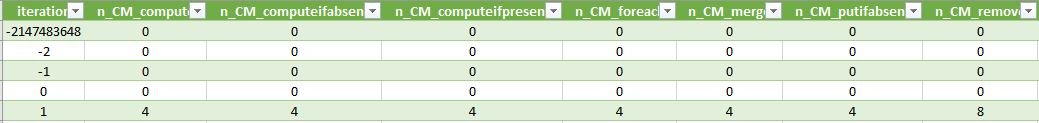
\includegraphics[scale=0.5]{Immagini/testing.JPG} 
    \caption{Metrics for testing of ConcurrentMap methos of CCOLL profiler module (PART 1).}
    \label{fig:fig1}
\end{figure}
\begin{figure}[h]
    \centering
    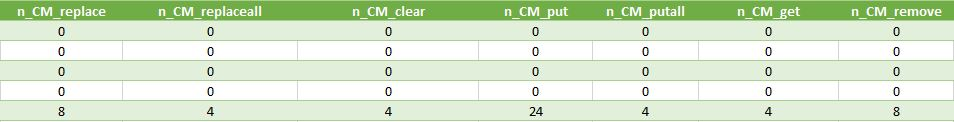
\includegraphics[scale=0.5]{Immagini/testing2.JPG} 
    \caption{Metrics for testing of ConcurrentMap methos of CCOLL profiler module (PART 2).}
    \label{fig:fig1}
\end{figure}


\chapter{Evaluation}

\section{Methodology and Setup}
\large
We present the evaluation of our profiler for \textit{Renaissance}: a well-established benchmark suite containing a range of modern workloads specifically designed for the JVM. Benchmarks workloads strongly implement concurrency, thus the choice of instrumenting this benchmark suite. We collect metrics on the methods usage frequency of concurrent libraries used by the benchmarks contained in the Renaissance suite. We analyse the results, identifying and discussing popularity of each library. Furthermore, we analyze profiler overhead, by collecting data regarding execution time of instrumented benchmarks compared with regular benchmarks execution. 

We conduct our evaluation on a machine equipped with an Intel Core i7-7700HQ (2.80 GHz) processor with 4 physical cores and 16 GB of RAM, running under Ubuntu 16.04.1 LTS. In order to reduce OS-layer metrics perturbation, no other intensive computations are executed during profiling. To minimize non determinism factors introduced by hidden OS processes execution, each execution of instrumented and non-instrumented benchmark is repeated 5 times. Collected data is grouped and averaged, and then used for the analysis. Table 5.1 lists the workloads included in the Renaissance benchmark suite, alongside a brief description, and the number of default warm-up iterations.

\begin{table}
\centering
\caption{Renaissance workloads considered in the dissertation. Benchmark description is taken from \url{https://renaissance.dev/docs}}
\begin{tabularx}{\textwidth}{|l|X|c|}
\hline
Benchmark&Description&Iterations\\
\hline
AKKA-UCT&Runs the Unbalanced Cobwebbed Tree actor workload in Akka.&24\\
ALS&Runs the ALS algorithm from the Spark MLlib.&30\\
CHI-SQUARE&Runs the chi-square test from Spark MLlib.&60\\
DB-SHOOTOUT&Executes a shootout test using several in-memory databases.&16\\
DEC-TREE&Runs the Random Forest algorithm from Spark MLlib.&40\\
DOTTY&Runs the Dotty compiler on a set of source code files.&50\\
FINAGLE-CHIRPER&Simulates a microblogging service using Twitter Finagle.&90\\
FINAGLE-HTTP&Sends many small Finagle HTTP requests to a Finagle HTTP server and awaits response.&12\\
FJK-MEANS&Runs the k-means algorithm using the fork/join framework.&30\\
FUTURE-GENETIC&Runs a genetic algorithm using the Jenetics library and futures.&50\\
GAUSS-MIX&Computes a Gaussian mixture model using expectation-maximization.&40\\
LOG-REGRESSION&Runs the logistic regression workload from the Spark MLlib.&20\\
MNEMONICS&Solves the phone mnemonics problem using JDK streams.&16\\
MOVIE-LENS&Recommends movies using the ALS algorithm.&20\\
NAIVE-BAYES&Runs the multinomial naive Bayes algorithm from the Spark MLlib.&30\\
NEO4J-ANALYTICS&Executes Neo4J graph queries against a movie database.&20\\
PAGE-RANK&Runs a number of PageRank iterations, using RDDs.&20\\
PAR-MNEMONICS&Solves the phone mnemonics problem using parallel JDK streams.&16\\
PHILOSOPHERS&Solves a variant of the dining philosophers problem using ScalaSTM.&30\\
REACTORS	&Runs benchmarks inspired by the Savina microbenchmark workloads in a sequence on Reactors.IO.	&10	\\
RX-SCRABBLE	&Solves the Scrabble puzzle using the Rx streams.	&80	\\
SCALA-DOKU	&Solves Sudoku Puzzles using Scala collections.	&20	\\
SCALA-KMEANS	&Runs the K-Means algorithm using Scala collections. 	&50	\\
SCALA-STM-BENCH	&Runs the stmbench7 benchmark using ScalaSTM.	&60	\\
SCRABBLE	&Solves the Scrabble puzzle using JDK Streams.	&50	\\
\hline
\end{tabularx}
\end{table}%

\begin{figure}
    \centering
    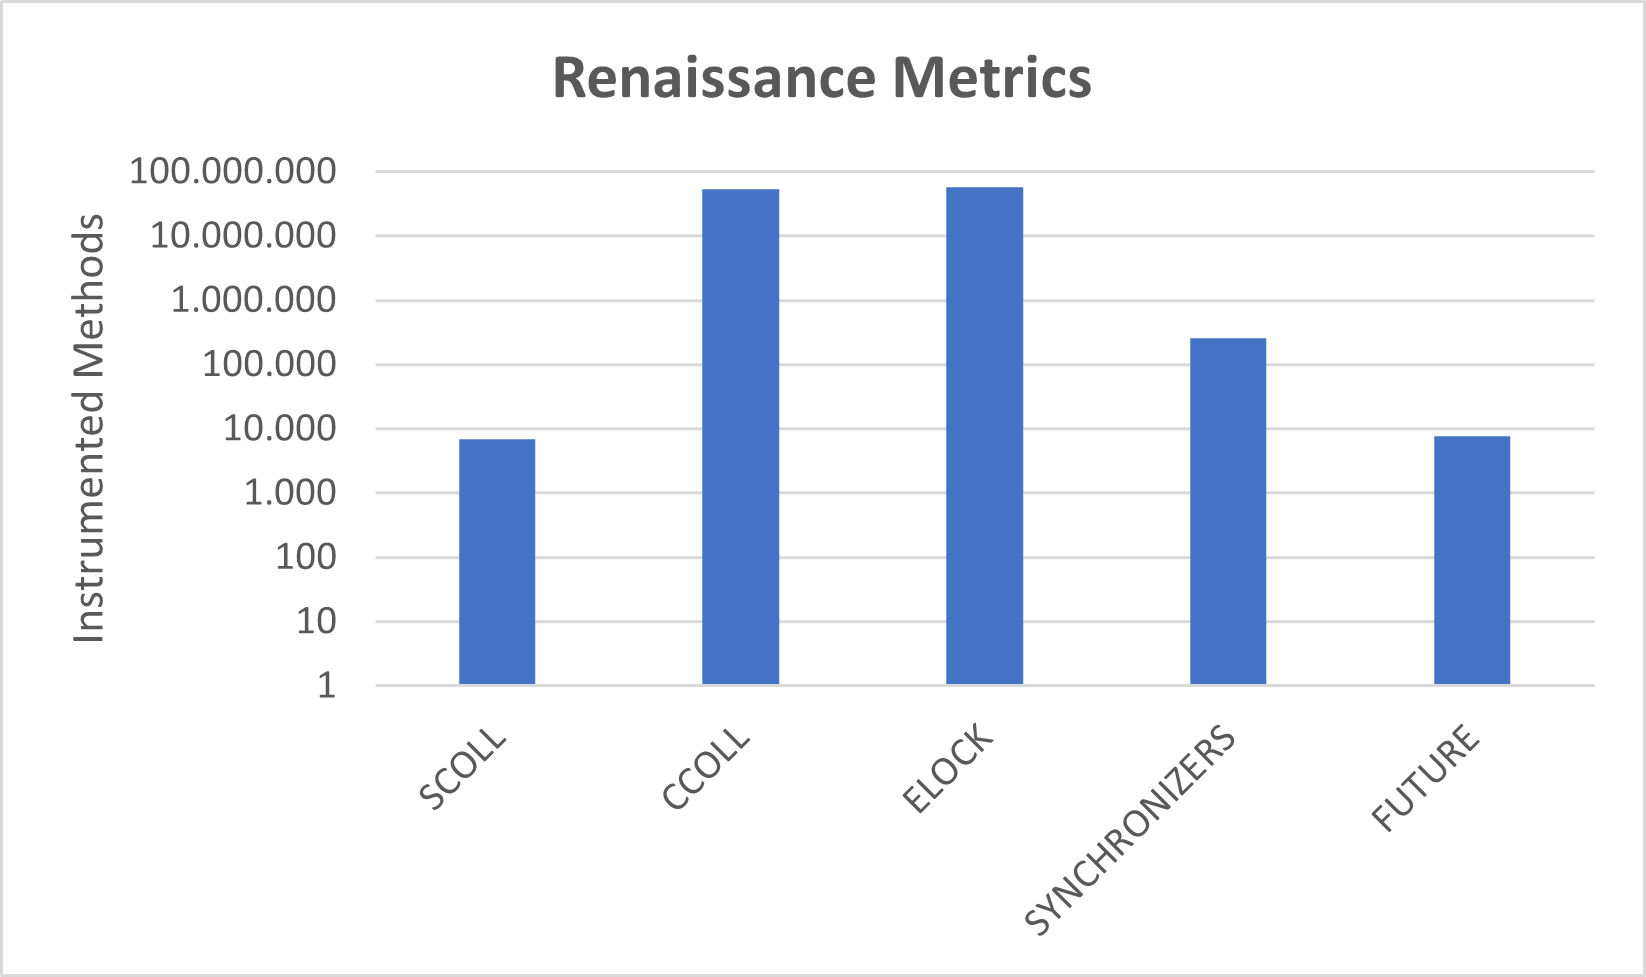
\includegraphics[scale=0.7]{Immagini/final metrics.png} 
    \caption{Method usage frequencies divided by Profiler modules.}
    \label{fig:fig1}
\end{figure}

\begin{figure}
    \centering
    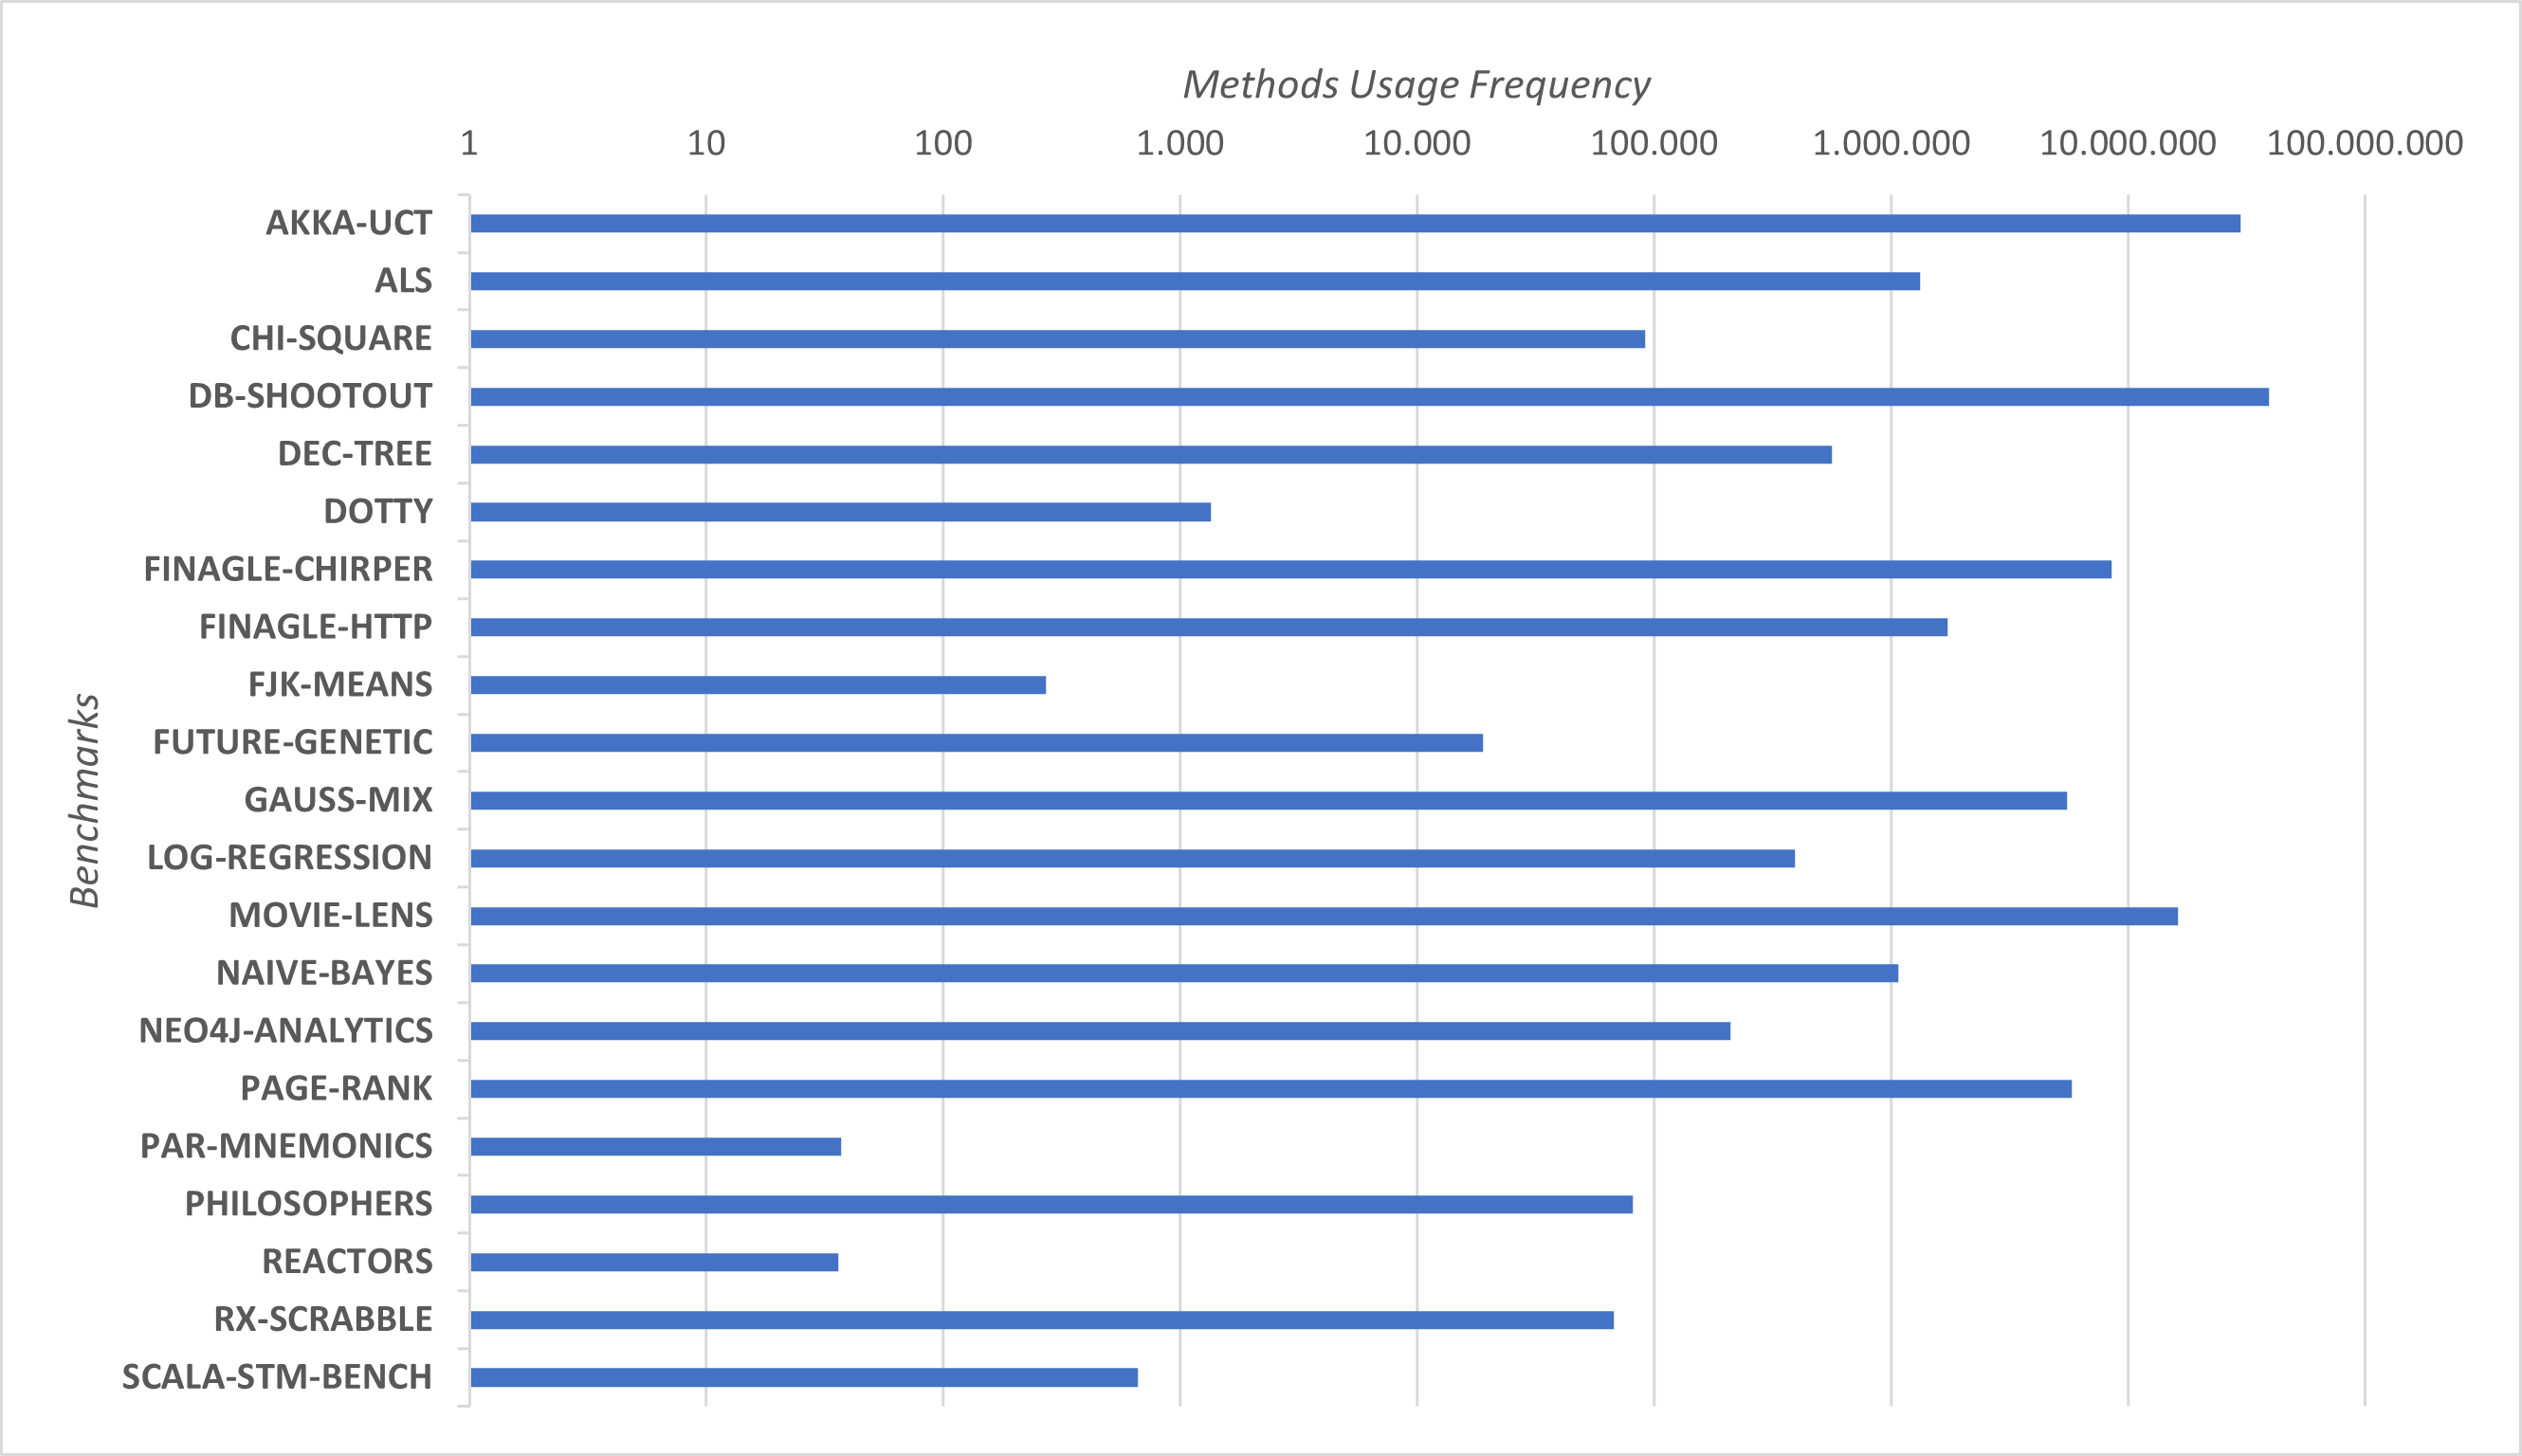
\includegraphics[scale=0.7]{Immagini/finalmetricsbenchm.png} 
    \caption{Method usage frequencies divided by benchmarks.}
    \label{fig:fig1}
\end{figure}

\section{Metrics}
We present the data collected on the frequency of methods usage of concurrent libraries of the JCL by profiling the Renaissance benchmark suite. This data is, to the best of our knowledge, completely novel. For every profiler module, we gather the metrics output, which is a set of comma-separated values file of benchmark executions, containing data of methods usage frequencies divided by benchmark iterations and frequency counters. For every benchmark execution, we select the data contained in the last iteration, which is the one executed after all warm-up iterations, thus containing the most accurate analysis. Table 5.2 lists the number of profiled methods divided by benchmarks and profiler modules. Benchmarks with no concurrent methods usage (MNEMONICS, SCALA-DOKU, SCALA-KMEANS, and SCRABBLE) are not included in the table. Tables 5.3, 5.4, 5.5, 5.6, and 5.7 list the number of profiled methods divided by methods usage frequency counter for each profiler module. Frequency counters scoring zero, thus counters for concurrent methods of interest that aren't used by none of the benchmarks, are not included in the table. Figures 5.1 and 5.2 are graphs representing overall profiled methods frequencies. The first one divides data by profiler modules, while the second one divided data by benchmarks. Both graphs use a logarithmic scale to represent the number of profiled methods. We make this choice in order to increase readability, due to the varying range of data, which fluctuates between \(10^1\) to \(10^7\).

Overall, the most used libraries are the concurrent collections (CCOLL) and the explicit locks (ELOCK) with more than \(5*10^7\) method calls each. Synchronized collections (SCOLL) and asynchronous computation libraries (FUTURE) are far less used, with less than \(8*10^3\) method calls each. A bit more popular, but still much less used in comparison with the first two, are the synchronizers (SYNCHRONIZERS) with less than \(3*10^3\) method usage.

Moreover, the benchmarks that have the highest frequency of concurrent methods usage are the AKKA-UCT, DB-SHOOTOUT, and MOVIE-LENS, with more than \(10^7\) method calls each, followed by ALS, FINAGLE-CHIRPER, FINAGLE-HTTP, GAUSS-MIX, NAIVE-BAYES, and PAGE-RANK benchmarks, with more than \(10^6\) method calls each. CHI-SQUARE, DEC-TREE, FUTURE-GENETIC, LOG-REGRESSION, NEO4J-ANALYTICS, PHILOSOPHERS, and RX-SCRABBLE benchmarks range their frequencies between \(10^4\) and \(10^5\), while the remaining benchmarks DOTTY, FJK-MEANS, PAR-MNEMONICS, REACTORS, and SCALA-STM-BENCH score \(10^3\) or less. 


\begin{table}
\centering
\caption{Number of profiled methods divided by benchmark and profiler module.}
{\scriptsize
\begin{tabular}{|c|c|c|c|c|c||c|}
\hline
\textbf{Benchmark}	&	\textbf{SCOLL}	&	\textbf{CCOLL}	&	\textbf{ELOCK}	&	\textbf{SYNCHRONIZERS}	&	\textbf{FUTURE}	& \textbf{Total} \\ 
\hline
AKKA-UCT	&	 -   	&	 13.999.691 	&	 15.725.546 	&	 21 	&	 -   	&	 \textbf{29.725.258} 	 \\ 
ALS	&	 10 	&	 1.277.691 	&	 42.746 	&	 766 	&	 365 	&	 \textbf{1.321.578} 	 \\ 
CHI-SQUARE	&	 13 	&	 87.659 	&	 4.058 	&	 52 	&	 17 	&	 \textbf{91.799} 	 \\ 
DB-SHOOTOUT	&	 -   	&	 2.028.401 	&	 37.174.198 	&	 -   	&	 -   	&	 \textbf{39.202.599} 	 \\ 
DEC-TREE	&	 898 	&	 515.139 	&	 47.218 	&	 295 	&	 91 	&	 \textbf{563.641} 	 \\ 
DOTTY	&	 -   	&	 - 	&	 1.344 	&	 -   	&	 -   	&	 \textbf{1.344} 	 \\ 
FINAGLE-CHIRPER	&	 -   	&	 7.572.113 	&	 951.216 	&	 19.996 	&	 1.968 	&	 \textbf{8.545.293} 	 \\ 
FINAGLE-HTTP	&	 -   	&	 193.073 	&	 1.344.980 	&	 191.993 	&	 32 	&	\textbf{ 1.730.078} 	 \\ 
FJK-MEANS	&	 -   	&	 - 	&	 270 	&	 -   	&	 -   	&	 \textbf{270} 	 \\ 
FUTURE-GENETIC	&	 -   	&	 15 	&	 18.900 	&	 -   	&	 -   	&	 \textbf{18.915} 	 \\ 
GAUSS-MIX	&	 148 	&	 5.513.815 	&	 16.046 	&	 426 	&	 159 	&	 \textbf{5.530.594} 	 \\ 
LOG-REGRESSION	&	 4.699 	&	 275.506 	&	 110.015 	&	 448 	&	 120 	&	 \textbf{390.788} 	 \\ 
MOVIE-LENS	&	 545 	&	 15.421.684 	&	 730.055 	&	 10.846 	&	 4.708 	&	\textbf{ 16.167.838} 	 \\ 
NAIVE-BAYES	&	 472 	&	 1.035.303 	&	 30.843 	&	 222 	&	 39 	&	\textbf{ 1.066.879} 	 \\ 
NEO4J-ANALYTICS	&	 -   	&	 202.945 	&	 5.920 	&	 -   	&	 10 	&	 \textbf{208.875} 	 \\ 
PAGE-RANK	&	 -   	&	 5.617.135 	&	 176.894 	&	 120 	&	 24 	&	\textbf{ 5.794.173 }	 \\ 
PAR-MNEMONICS	&	 -   	&	 37 	&	 -   	&	 -   	&	 -   	&	 \textbf{37} 	 \\ 
PHILOSOPHERS	&	 -   	&	 57.177 	&	 23.913 	&	 -   	&	 -   	&	 \textbf{81.090} 	 \\ 
REACTORS	&	 -   	&	 - 	&	 36 	&	 -   	&	 -   	&	 \textbf{36} 	 \\ 
RX-SCRABBLE	&	 -   	&	 311 	&	 34.361 	&	 32.968 	&	 155 	&	 \textbf{67.795} 	 \\ 
SCALA-STM-BENCH	&	 -   	&	 659 	&	 -   	&	 -   	&	 -   	&	 \textbf{659} 	 \\ 
\hline													
\hline													
\textbf{Total}	&  \textbf{	 6.785 	} &  \textbf{	 53.798.362 	} &  \textbf{	 56.438.559 	} &  \textbf{	 258.153 	} &  \textbf{	7688	} &  \textbf{	 110.509.539 	 }\\ 
\hline													
\end{tabular}
}
\end{table}%


\subsection{SCOLL Metrics}
The synchronized collections are one of the least used libraries of Renaissance. SCOLL profiler module, in fact, identifies less than \(7*10^3\) method calls, and out of 57 instrumented methods, only 2 are actually used inside the Renaissance benchmark suite, and they are part of the \textit{SynchronizedMap} class:
\begin{itemize}
    \item V get(Object key)
    \item V put(K key, V value)
\end{itemize}
 This excludes usage of all other structurally modifying methods of the same class (e.g. \textit{remove}, \textit{replace}, \textit{compute}, \textit{clear}, etc.) suggesting a basic utilisation of the structure, where elements are simply inserted and read from a synchronizedMap, but never modified or removed. All other classes of the library (i.e. \textit{SynchronizedList}, \textit{SynchronizedSortedMap}, \textit{SynchronizedNavigableMap}, \textit{SynchronizedSortedSet}, \textit{SynchronizedNavigableSet}) are also never used.
 
 Benchmarks that utilize synchronized collections are only 7 out of 25, and FINAGLE-CHIRPER and MOVIE-LENS benchmarks alone covers more than \(2/3\) of overall method usage. Once again, this information suggests very scarce exploitation of the synchronized collections library by the Renaissance benchmark suite.
 
 
\begin{table}
\centering
\caption{Number of profiled methods divided by method usage frequency counter for the SCOLL profiler module.}
\begin{tabular}{|c|c|}
\hline
\textbf{Frequency Counter} & \textbf{# Profiled methods} \\
\hline
n\_SMap\_get	&	5.391	 \\ 
n\_SMap\_put	&	1.394	 \\ 
\hline			
\hline			
\textbf{Total}	&  \textbf{	6.785	 }\\ 
\hline			
\end{tabular}
\end{table}%


\subsection{CCOLL Metrics}
The concurrent collections are one of the most used libraries of Renaissance. CCOLL profiler module, in fact, identifies more than \(5*10^7\) method calls. However, usage is not very diversified, and out of 63 instrumented methods, only 14 (actually 18, but 4 methods are merged with others in single frequency counters) are used inside the Renaissance benchmark suite, and they are part of the \textit{ConcurrentMap} and \textit{BlockingQueue} interfaces:
\begin{itemize}
    \item BlockingQueue<E>:
    \begin{itemize}
        \item boolean add(E e)
        \item boolean offer(E e)
        \mbox{}\\ boolean offer(E e, long timeout, TimeUnit unit)
        \item E poll(long timeout, TimeUnit unit)
        \mbox{}\\ E poll()
        \item void put(E e)
        \item boolean remove(Object o)
        \item E take()
    \end{itemize}
    \item ConcurrentMap<K,V>:
    \begin{itemize}    
    \item   V computeIfAbsent(K key, Function<? super K,? extends V> mappingFunction)
    \item   V computeIfPresent(K key, BiFunction<? super K,? super V,? extends V> remappingFunction)
    \item   V putIfAbsent(K key, V value)
    \item   boolean remove(Object key, Object value)
    \mbox{}\\      V remove(Object key)
    \item   V replace(K key, V value)
    \mbox{}\\      boolean replace(K key, V oldValue, V newValue)
    \item   void clear()
    \item   V put(K key, V value)
    \item   V get(Object key)
    \end{itemize}
\end{itemize}
 Detected method usage represents an exhaustive variety of functionality utilization for both classes, with operations of data insertion, modification, removal and reading. However, none of the other classes (i.e. \textit{BlockingDeque}, \textit{TransferQueue}, \textit{ArrayBlockingQueue}, \textit{DelayQueue}, \textit{LinkedBlockingQueue}, \textit{PriorityBlockingQueue}, \textit{SynchronousQueue}, \textit{LinkedBlockingDeque}, \textit{LinkedTransferQueue}, \textit{ConcurrentNavigableMap}, \textit{ConcurrentHashMapare}, \textit{ConcurrentSkipListMap}, \textit{CopyOnWriteArrayList}, \textit{ConcurrentSkipListSet}, and \textit{CopyOnWriteArraySet}) are utilized by the Renaissance benchmark suite. This does not mean that none of these classes are never implemented inside the code. In fact, some of them are necessarily used, since \textit{BlockingQueue} and \textit{ConcurrentMap} are both interfaces, thereby not instantiable. However, none of the class specific methods for any sub-typing class is utilized. This suggests a standard usage of the library, where only methods of the main interfaces are used.
 
 It is also of importance to notice that almost \(95\%\) of profiled method calls come from the \textit{get} method of class \textit{ConcurrentMap}. This means that Renaissance workloads for CCOLL library mainly focus on data reading.
 
 Benchmarks that utilize synchronized collections are 18 out of 25, and usage frequency is quite diversified between them. This information suggests a rather strong exploitation of the concurrent collections library inside the Renaissance workloads.

\begin{table}
\centering
\caption{Number of profiled methods divided by method usage frequency counter for the CCOLL profiler module.}
\begin{tabular}{|c|c|}
\hline
\textbf{Frequency Counter} & \textbf{# Profiled Methods} \\
\hline
n\_CM\_computeifabsent	&	 4.350 	 \\ 
n\_CM\_computeifpresent	&	 992 	 \\ 
n\_CM\_putifabsent	&	 929.078 	 \\ 
n\_CM\_remove	&	 23.462 	 \\ 
n\_CM\_replace	&	 10 	 \\ 
n\_CM\_clear	&	 141 	 \\ 
n\_CM\_put	&	 1.506.220 	 \\ 
n\_CM\_get	&	 51.252.829 	 \\ 
n\_BQ\_take	&	 21.226 	 \\ 
n\_BQ\_remove	&	 5.280 	 \\ 
n\_BQ\_put	&	 9.594 	 \\ 
n\_BQ\_poll	&	 14.130 	 \\ 
n\_BQ\_offer	&	 25.587 	 \\ 
n\_BQ\_add	&	 5.437 	 \\ 
\hline
\hline
\textbf{Total}	&	  \textbf{53.798.336}    	 \\ 
\hline
\end{tabular}
\end{table}%


\subsection{ELOCK Metrics}
The explicit locks library is the most used library of Renaissance. ELOCK profiler module  identifies more than \(5*10^7\) method calls. Usage is quite diversified, and out of 26 instrumented methods, half of them are used inside the Renaissance benchmark suite, and they are part of the \textit{Lock}, \textit{ReadWriteLock}, \textit{Condition}, \textit{AbstractQueuedSynchronizer}, and \textit{LockSupport} classes:
\begin{itemize}
\item Lock:
    \begin{itemize}
        \item   void lock()
         \mbox{}\\ void lockInterruptibly()
        \item   Condition newCondition()
        \item   boolean tryLock()
         \mbox{}\\ boolean tryLock(long time, TimeUnit unit)
        \item   void unlock()
    \end{itemize}
\item ReadWriteLock:
\begin{itemize}
    \item   Lock readLock()
    \item   Lock writeLock()
\end{itemize}

\item Condition:
    \begin{itemize}
        \item   void await()
         \mbox{}\\ boolean await(long time, TimeUnit unit)
         \mbox{}\\ long awaitNanos(long nanosTimeout)
         \mbox{}\\ void awaitUninterruptibly()
         \mbox{}\\ boolean awaitUntil(Date deadline)
        \item   void signal()
    \end{itemize}

\item AbstractQueuedSynchronizer:
    \begin{itemize}
        \item   void acquire(int arg)
         \mbox{}\\ void acquireInterruptibly(int arg)
         \mbox{}\\ void acquireShared(int arg)
         \mbox{}\\ void acquireSharedInterruptibly(int arg)
        \item   boolean release(int arg)
         \mbox{}\\ boolean releaseShared(int arg)
        \item   boolean tryAcquireNanos(int arg, long nanosTimeout)
         \mbox{}\\ boolean tryAcquireSharedNanos(int arg, long nanosTimeout)
    \end{itemize}

\item LockSupport:
    \begin{itemize}
        \item   static void park()
         \mbox{}\\ static void park(Object blocker)
         \mbox{}\\ static void parkNanos(long nanos)
         \mbox{}\\ static void parkNanos(Object blocker, long nanos)
         \mbox{}\\ static void parkUntil(long deadline)
         \mbox{}\\ static void parkUntil(Object blocker, long deadline)
        \item   static void unpark(Thread thread)
    \end{itemize}
\end{itemize}
 Detected method usage represents an exhaustive variety of functionality utilization for all the classes listed above. Despite the fact that none of the remaining instrumented classes (i.e. \textit{AbstractQueuedLongSynchronizer}, \textit{ReentrantLock}, and \textit{UnsafeStampedLock}) are utilized by the Renaissance benchmark suite, the latter still implement most of the functionalities of the explicit locks library. Detected methods frequencies are distributed quite well, ranging from \(10^3\) to \(10^7\). Thus, we can conclude that Renaissance benchmark workloads make thorough usage of explicit locks.
 
 The number of benchmarks that utilize explicit locks is the highest of all profiler modules, and they are 19 out of 25. However method usage frequency is not much diversified and AKKA-UCT and DB-SHOOTOUT benchmarks alone covers almost \(95\%\) of method usage of the library. Compared with the concurrent collection library, we can say that it is less widely used. Thus, less popular.
 
 \begin{table}
\centering
\caption{Number of profiled methods divided by method usage frequency counter for the ELOCK profiler module.}
\begin{tabular}{|c|c|}
\hline
\textbf{Frequency Counter} & \textbf{# Profiled Methods} \\
\hline
n\_Lock\_lock	&	 12.422.374 	 \\ 
n\_Lock\_newCondition	&	 2.970 	 \\ 
n\_Lock\_tryLock	&	 6.124.938 	 \\ 
n\_Lock\_unlock	&	 17.047.286 	 \\ 
n\_RWLock\_readLock	&	 16.390.156 	 \\ 
n\_RWLock\_writeLock	&	 1.000.000 	 \\ 
n\_Condition\_await	&	 17.775 	 \\ 
n\_Condition\_signal	&	 58.669 	 \\ 
n\_AQS\_acquire	&	 949.228 	 \\ 
n\_AQS\_release	&	 1.099.315 	 \\ 
n\_AQS\_tryAcquire	&	 110.822 	 \\ 
n\_LockSupport\_park	&	 607.513 	 \\ 
n\_LockSupport\_unpark	&	 607.513 	 \\ 
\hline			
\hline			
\textbf{Total}	&  \textbf{	 56.438.559 	 }\\ 
\hline			
\end{tabular}
\end{table}%


 
 \subsection{SYNCHRONIZERS Metrics}
The synchronizers library is one of the least used libraries of Renaissance. SYNCHRONIZERS profiler module identifies less than \(3*10^5\) method calls, and out of 16 instrumented methods, only 4 are used inside the Renaissance benchmark suite workloads, and they are part of the \textit{Semaphore} and \textit{CountDownLatch} classes:
\begin{itemize}
    \item Semaphore:
    \begin{itemize}
        \item   void acquire()
        \mbox{}\\ void acquire(int permits)
        \mbox{}\\ void acquireUninterruptibly()
        \mbox{}\\ void acquireUninterruptibly(int permits)
        \item   void release()
        \mbox{}\\ void release(int permits)
        \end{itemize}
    \item CountDownLatch:
        \begin{itemize}
        \item   void await()
        \mbox{}\\ boolean await(long timeout, TimeUnit unit)
        \item   void countDown()
        \end{itemize}
\end{itemize}
Both classes are thoroughly used inside Renaissance workloads, even though frequency remain quite low. ranging between \(10^3\) to \(10^5\) method usages. This excludes utilization of all other classes of the library (i.e. \textit{CyclicBarrier}, \textit{Phaser}, and \textit{Exchanger}). Benchmarks that utilize synchronizers are 12 out of 25, but the single FINAGLE-CHIRPER benchmark alone covers more than \(3/5\) of overall method usage. Both information suggests a low exploitation of synchronizers library by the Renaissance benchmark suite.

\begin{table}
\centering
\caption{Number of profiled methods divided by method usage frequency counter for the SYNCHRONIZERS profiler module.}
\begin{tabular}{|c|c|}
\hline
\textbf{Frequency Counter} & \textbf{# Profiled Methods} \\
\hline
n\_Semaphore\_acquire	&	 6.588 	 \\ 
n\_Semaphore\_release	&	 6.587 	 \\ 
n\_CTL\_await	&	 105.999 	 \\ 
n\_CTL\_countDown	&	 138.979 	 \\ 
\hline			
\hline			
\textbf{Total}	&  \textbf{	 258.153 	 }\\ 
\hline			
\end{tabular}
\end{table}%

 \subsection{FUTURE Metrics}
Asynchronous computation is one of the least used libraries of Renaissance. FUTURE profiler module, in fact, identifies less than \(8*10^3\) method calls, and out of 25 instrumented methods, only 3 (actually 4, but both get method are merged inside the same frequency counter) are used inside the Renaissance benchmark suite, and they are part of the \textit{Future} interface, and its sub-type \textit{RunnableFuture} interface:
\begin{itemize}
    \item Future<V>:
    \begin{itemize}
        \item   boolean cancel(boolean mayInterruptIfRunning)
        \item   V get()
        \mbox{}\\ V get(long timeout, TimeUnit unit)
    \end{itemize}
    \item RunnableFuture<V>:
    \begin{itemize}
        \item   void run()
    \end{itemize}
\end{itemize}
 This excludes usage of all other classes of the library (i.e. \textit{CompletionStage} and \textit{CompletableFuture}) suggesting a basic utilisation of the structure, where future computation are received, run and sometimes cancelled.
 
 Benchmarks that utilize synchronized collections are 12 out of 25, and LOG-REGRESSION benchmark alone covers more than \(85\%\) of overall method usage. Once again, this information suggests very scarce exploitation of asynchronous computation library by the Renaissance benchmark suite.


\begin{table}
\centering
\caption{Number of profiled methods divided by method usage frequency counter for the FUTURE profiler module.}
\begin{tabular}{|c|c|}
\hline
\textbf{Frequency Counter} & \textbf{# Profiled Methods} \\
\hline
n\_Future\_get	&	 4.328 	 \\ 
n\_Future\_cancel	&	 2.212 	 \\ 
n\_RunnableFuture\_run	&	 1.148 	 \\ 
\hline			
\hline			
\textbf{Total}	&  \textbf{	 7.688 	 }\\ 
\hline		
\end{tabular}
\end{table}%

\section{Performance}
In this section we compare running time of each profiler module with the standard execution of the Renaissance benchmark suite. In order to do so, we calculate average execution time, with correspondent 95\% confidence intervals, of 30 steady-state runs (5 for each profiler modules, plus 5 for standard Renaissance execution). Figure 5.3 represents the comparison of all profiler module with the standard renaissance execution time expressed in seconds. We also analyse the overhead, defined as the execution time of the instrumented workloads divided by the execution time of the standard workload. For each run, we determine the corresponding overhead. After 5 run, we average them together with 95\% confidence intervals. In table 5.8 we represent the overhead calculated for each profiler module, while in tables 5.9 and 5.10 we also specify data for each benchmark execution.

ELOCK module is the fastest with 10.314s $\pm$ 60s of execution time and 1,01x of overhead. It is in average only 100s slower than the standard Renaissance execution, which scores 10.239s $\pm$ 101s. The slowest are the SCOLL, SYNCHRONIZERS, and FUTURE module, with respectively average execution times of 10.875s $\pm$ 302s, 11.003s $\pm$ 170s and 11.109s $\pm$ 169s, and overheads of 1,07x, 1,07x, and 1.08x. Only 184s slower then the fastest module is the CCOLL module which execution takes is average 10.498s $\pm$ 60s with an overhead of 1,03x. Interesting to notice is that the better performing modules are also the ones with the highest data collected on method usage frequencies. Logically, it should be the reverse, where the profiler modules collecting the largest number of information should also take the longest to execute. Profiled method frequency is also unrelated in the specific benchmark execution. For example, the FUTURE-GENETIC and the PAGE-RANK benchmarks scores an overhead of 4,73x and 3,00x respectively. However, both benchmarks don't profile any metrics for the synchronized collections. At the same time, the benchmark that uses SCOLL methods the most is LOG-REGRESSION which takes on average the same time to be executed on Renaissance, scoring an overload of 1,00x. We hypothesise the reasoning behind this behaviour with the fact that the instructions executed by our instrumentation are simple counters increases, thus not very expensive in term of memory usage. Actual benchmark workloads execution -thus profiler indipendent-, especially in a concurrent environment, may be the cause of differences in time execution.

Overall, execution time of all modules takes at most 860 additional seconds to complete compared with standard Renaissance, and overhead scores never more than 1.08x. Therefore proving the efficiency of our profiler.


\begin{figure}
    \centering
    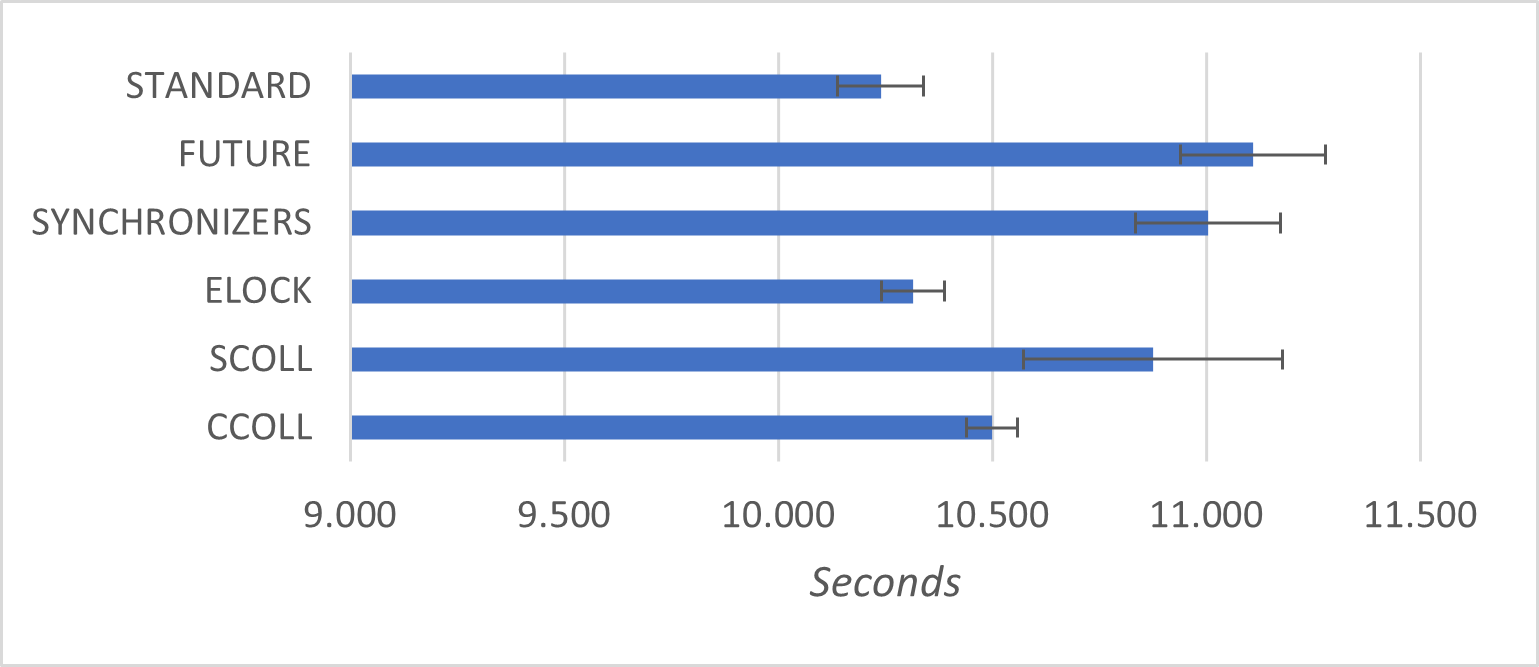
\includegraphics[scale=1]{Immagini/executiontime.png} 
    \caption{Average execution time, with 95\% confidence interval, of each profiler module and standard Renaissance benchmark suite execution.}
    \label{fig:fig1}
\end{figure}


\begin{table}
\centering
\caption{Average execution time and confidence interval expressed in seconds for each profiler module execution and standard Renaissance execution.}
\begin{tabular}{|c|c|}
\hline
		 & 	\textbf{	Overhead Factor	}		\\	
\textbf{	Benchmark	}&	\textbf{	 ($\pm$95\% conf.) 	}		\\	 \hline 
\textbf{	CCOLL	}&	 1,03 	$\pm$		 0,01 	\\	
\textbf{	SCOLL	}&	 1,07 	$\pm$		 0,04 	\\	
\textbf{	ELOCK	}&	 1,01 	$\pm$		 0,01 	\\	
\textbf{	SYNCHRONIZERS	}&	 1,07 	$\pm$		 0,01 	\\	
\textbf{	FUTURE	}&	 1,08 	$\pm$		 0,01 	\\	
\hline
\end{tabular}
\end{table}%

\begin{table}
\centering
\caption{Average overhead obtained on 5 steady-state runs with 95\% confidence intervals for profiler modules SCOLL, COLL, and ELOCK divided by benchmark.}
\begin{tabular}{|c|c|c|c|}
\hline
		 & 	\textbf{	SCOLL	}	 & 	\textbf{	CCOLL	}	 & 	\textbf{	ELOCK	}	\\
\textbf{	Benchmark	}& 	\textbf{	Overhead Factor	}	 & 	\textbf{	Overhead Factor	}	 & 	\textbf{	Overhead Factor	}	\\
&	\textbf{	 ($\pm$95\% conf.) 	}	 & 	\textbf{	 ($\pm$95\% conf.) 	}	 & 	\textbf{	 ($\pm$95\% conf.) 	}	\\

\hline
\textbf{	AKKA-UCT	}&	 1,00 	 $\pm$ 	 0,06 	 & 	 1,11 	 $\pm$ 	 0,02 	 & 	 1,00 	 $\pm$ 	 0,02 	\\
\textbf{	ALS	}&	 1,00 	 $\pm$ 	 0,07 	 & 	 1,00 	 $\pm$ 	 0,03 	 & 	 1,01 	 $\pm$ 	 0,01 	\\
\textbf{	CHI-SQUARE	}&	 2,00 	 $\pm$ 	 0,18 	 & 	 1,06 	 $\pm$ 	 0,05 	 & 	 1,00 	 $\pm$ 	 0,03 	\\
\textbf{	DB-SHOOTOUT	}&	 1,05 	 $\pm$ 	 0,07 	 & 	 1,00 	 $\pm$ 	 0,02 	 & 	 1,00 	 $\pm$ 	 0,01 	\\
\textbf{	DEC-TREE	}&	 1,00 	 $\pm$ 	 0,03 	 & 	 1,55 	 $\pm$ 	 0,10 	 & 	 1,31 	 $\pm$ 	 0,07 	\\
\textbf{	DOTTY	}&	 1,00 	 $\pm$ 	 0,05 	 & 	 1,08 	 $\pm$ 	 0,02 	 & 	 1,33 	 $\pm$ 	 0,07 	\\
\textbf{	FINAGLE-CHIRPER	}&	 1,47 	 $\pm$ 	 0,04 	 & 	 1,44 	 $\pm$ 	 0,10 	 & 	 1,15 	 $\pm$ 	 0,03 	\\
\textbf{	FINAGLE-HTTP	}&	 1,04 	 $\pm$ 	 0,04 	 & 	 1,06 	 $\pm$ 	 0,04 	 & 	 1,01 	 $\pm$ 	 0,02 	\\
\textbf{	FJK-MEANS	}&	 1,00 	 $\pm$ 	 0,02 	 & 	 1,07 	 $\pm$ 	 0,03 	 & 	 1,03 	 $\pm$ 	 0,03 	\\
\textbf{	FUTURE-GENETIC	}&	 4,73 	 $\pm$ 	 0,26 	 & 	 1,00 	 $\pm$ 	 0,02 	 & 	 1,08 	 $\pm$ 	 0,04 	\\
\textbf{	GAUSS-MIX	}&	 1,00 	 $\pm$ 	 0,06 	 & 	 1,31 	 $\pm$ 	 0,05 	 & 	 1,55 	 $\pm$ 	 0,09 	\\
\textbf{	LOG-REGRESSION	}&	 1,00 	 $\pm$ 	 0,05 	 & 	 1,14 	 $\pm$ 	 0,05 	 & 	 1,00 	 $\pm$ 	 0,02 	\\
\textbf{	MNEMONICS	}&	 1,00 	 $\pm$ 	 0,03 	 & 	 1,09 	 $\pm$ 	 0,04 	 & 	 1,04 	 $\pm$ 	 0,05 	\\
\textbf{	MOVIE-LENS	}&	 1,21 	 $\pm$ 	 0,06 	 & 	 1,04 	 $\pm$ 	 0,03 	 & 	 1,05 	 $\pm$ 	 0,03 	\\
\textbf{	NAIVE-BAYES	}&	 1,17 	 $\pm$ 	 0,05 	 & 	 1,00 	 $\pm$ 	 0,05 	 & 	 1,38 	 $\pm$ 	 0,09 	\\
\textbf{	NEO4J-ANALYTICS	}&	 1,20 	 $\pm$ 	 0,05 	 & 	 1,09 	 $\pm$ 	 0,04 	 & 	 1,00 	 $\pm$ 	 0,03 	\\
\textbf{	PAGE-RANK	}&	 3,00 	 $\pm$ 	 0,09 	 & 	 1,65 	 $\pm$ 	 0,12 	 & 	 1,68 	 $\pm$ 	 0,13 	\\
\textbf{	PAR-MNEMONICS	}&	 1,39 	 $\pm$ 	 0,12 	 & 	 1,19 	 $\pm$ 	 0,07 	 & 	 1,16 	 $\pm$ 	 0,09 	\\
\textbf{	PHILOSOPHERS	}&	 1,22 	 $\pm$ 	 0,06 	 & 	 1,44 	 $\pm$ 	 0,05 	 & 	 1,33 	 $\pm$ 	 0,07 	\\
\textbf{	REACTORS	}&	 1,00 	 $\pm$ 	 0,05 	 & 	 1,00 	 $\pm$ 	 0,03 	 & 	 1,00 	 $\pm$ 	 0,05 	\\
\textbf{	RX-SCRABBLE	}&	 1,00 	 $\pm$ 	 0,04 	 & 	 1,08 	 $\pm$ 	 0,06 	 & 	 1,00 	 $\pm$ 	 0,06 	\\
\textbf{	SCALA-DOKU	}&	 1,00 	 $\pm$ 	 0,05 	 & 	 1,04 	 $\pm$ 	 0,01 	 & 	 1,00 	 $\pm$ 	 0,03 	\\
\textbf{	SCALA-KMEANS	}&	 1,00 	 $\pm$ 	 0,03 	 & 	 1,05 	 $\pm$ 	 0,05 	 & 	 1,00 	 $\pm$ 	 0,03 	\\
\textbf{	SCALA-STM-BENCH	}&	 1,00 	 $\pm$ 	 0,08 	 & 	 1,00 	 $\pm$ 	 0,04 	 & 	 1,00 	 $\pm$ 	 0,04 	\\
\textbf{	SCRABBLE	}&	 1,00 	 $\pm$ 	 0,06 	 & 	 1,08 	 $\pm$ 	 0,05 	 & 	 1,00 	 $\pm$ 	 0,03 	\\
\hline
\end{tabular}
\end{table}%

\begin{table}
\centering
\caption{Average overhead obtained on 5 steady-state runs with 95\% confidence intervals for profiler modules SYNCHRONIZERS, and FUTURE divided by benchmark.}
\begin{tabular}{|c|c|c|}
\hline
		 & 	\textbf{	SYNCHRONIZERS	}	 & 	\textbf{	FUTURE	}	\\
\textbf{	Benchmark	}&	\textbf{	Overhead Factor	}	 & 	\textbf{	Overhead Factor	}	\\
		 & 	\textbf{	 ($\pm$95\% conf.) 	}	 & 	\textbf{	 ($\pm$95\% conf.) 	}	\\
		 
\hline
\textbf{	AKKA-UCT	}&	 1,14 	 $\pm$ 	 0,04 	 & 	 1,28 	 $\pm$ 	 0,06 	\\
\textbf{	ALS	}&	 1,06 	 $\pm$ 	 0,02 	 & 	 1,00 	 $\pm$ 	 0,02 	\\
\textbf{	CHI-SQUARE	}&	 1,11 	 $\pm$ 	 0,04 	 & 	 1,40 	 $\pm$ 	 0,06 	\\
\textbf{	DB-SHOOTOUT	}&	 1,00 	 $\pm$ 	 0,04 	 & 	 1,00 	 $\pm$ 	 0,02 	\\
\textbf{	DEC-TREE	}&	 1,13 	 $\pm$ 	 0,04 	 & 	 1,08 	 $\pm$ 	 0,04 	\\
\textbf{	DOTTY	}&	 1,43 	 $\pm$ 	 0,07 	 & 	 1,09 	 $\pm$ 	 0,02 	\\
\textbf{	FINAGLE-CHIRPER	}&	 1,31 	 $\pm$ 	 0,10 	 & 	 1,51 	 $\pm$ 	 0,08 	\\
\textbf{	FINAGLE-HTTP	}&	 1,04 	 $\pm$ 	 0,03 	 & 	 1,15 	 $\pm$ 	 0,03 	\\
\textbf{	FJK-MEANS	}&	 1,04 	 $\pm$ 	 0,06 	 & 	 1,06 	 $\pm$ 	 0,05 	\\
\textbf{	FUTURE-GENETIC	}&	 1,00 	 $\pm$ 	 0,02 	 & 	 1,18 	 $\pm$ 	 0,06 	\\
\textbf{	GAUSS-MIX	}&	 1,29 	 $\pm$ 	 0,02 	 & 	 1,54 	 $\pm$ 	 0,08 	\\
\textbf{	LOG-REGRESSION	}&	 1,10 	 $\pm$ 	 0,02 	 & 	 1,02 	 $\pm$ 	 0,03 	\\
\textbf{	MNEMONICS	}&	 1,00 	 $\pm$ 	 0,02 	 & 	 1,01 	 $\pm$ 	 0,03 	\\
\textbf{	MOVIE-LENS	}&	 1,09 	 $\pm$ 	 0,01 	 & 	 1,07 	 $\pm$ 	 0,04 	\\
\textbf{	NAIVE-BAYES	}&	 1,26 	 $\pm$ 	 0,07 	 & 	 1,32 	 $\pm$ 	 0,08 	\\
\textbf{	NEO4J-ANALYTICS	}&	 1,14 	 $\pm$ 	 0,04 	 & 	 1,34 	 $\pm$ 	 0,09 	\\
\textbf{	PAGE-RANK	}&	 1,71 	 $\pm$ 	 0,13 	 & 	 1,53 	 $\pm$ 	 0,11 	\\
\textbf{	PAR-MNEMONICS	}&	 1,20 	 $\pm$ 	 0,06 	 & 	 1,18 	 $\pm$ 	 0,08 	\\
\textbf{	PHILOSOPHERS	}&	 1,60 	 $\pm$ 	 0,07 	 & 	 1,78 	 $\pm$ 	 0,12 	\\
\textbf{	REACTORS	}&	 1,00 	 $\pm$ 	 0,05 	 & 	 1,00 	 $\pm$ 	 0,04 	\\
\textbf{	RX-SCRABBLE	}&	 1,16 	 $\pm$ 	 0,04 	 & 	 1,15 	 $\pm$ 	 0,04 	\\
\textbf{	SCALA-DOKU	}&	 1,00 	 $\pm$ 	 0,02 	 & 	 1,06 	 $\pm$ 	 0,04 	\\
\textbf{	SCALA-KMEANS	}&	 1,05 	 $\pm$ 	 0,03 	 & 	 1,00 	 $\pm$ 	 0,02 	\\
\textbf{	SCALA-STM-BENCH	}&	 1,00 	 $\pm$ 	 0,06 	 & 	 1,00 	 $\pm$ 	 0,08 	\\
\textbf{	SCRABBLE	}&	 1,00 	 $\pm$ 	 0,03 	 & 	 1,01 	 $\pm$ 	 0,02 	\\

\hline
\end{tabular}
\end{table}%



\chapter{Conclusion}

Nowadays, multi-core architectures represent the norm. Therefore, concurrent programming has become fundamental to enhance performance and build competitive software. Programming languages generally offer constructs to facilitate approaching concurrency. However, despite the abundance of available libraries, there are very few studies on the frequency in which they are used. This information may turn out to be very useful in a variety of contexts, such as compiler development, libraries implementation and research purposes.

This dissertation proposes a novel methodology of collecting method and class usage frequency information for concurrent libraries of the JCL. We present a new profiler that, relying on AOP principles and out-of-process bytecode instrumentation, allows efficient and accurate profiling of concurrent applications running on the JVM. This tool is specifically designed to analyze usage of concurrent and synchronized collections, explicit locks, synchronizers, and asynchronous computation constructs, by collecting usage frequencies for selected methods of interest of such libraries. We also present a practical usage of the profiler for the Renaissance benchmark suite, providing the scientific community with novel insights on this established and reliable set of benchmarks, while also proving the efficiency of our tool.

\section{Limitation}
As previously discussed, our profiler works by injecting instrumentation code inside the target applications. This operation is intrinsically modifying as regards the analyzed application code. Concomitant therewith, injected instrumentation code may influence thread scheduling or produce measurement perturbation during target application execution, therefore providing biased metrics as results. We took several measures in order to minimize this problem, such as the usage of thread-local variables to avoid the need of synchronization, and the ShadowVM which allows performing analysis operations on a separate JVM from the one used for the target application execution. These precautions result in an low overhead and consequent efficient profiling, thus reducing changes of significant measurement perturbations.

Moreover, when working with time metrics for software evaluation, instristic biases are inevitable. Thus, our evaluation on the performance for standard benchmarks and profiler modules execution may also be susceptible of biased results. This is mainly caused by the architecture of the machine of choice used to perform the analysis and the non-determinism principles onto which concurrency is based. We took several measures to guarantee -as much as possible- accuracy in our evaluation. We ran each operation on the same machine, which was specifically set-up to only focus on this task. Thus, we made sure that no other execution was running at the time, providing an environment that was controlled to the greatest extent possible. Also, each standard benchmark and profiler module execution was reaped 5 times, and the evaluation was conducted on the average values, with corresponding confidence intervals. Hence, statistically reducing randomness factors of program execution.



\section{Future Work}
Future developments of our work include using our tool to profile other benchmark suites, in order to collect more data on the usage of concurrent libraries, improving analyses, and overall possible exploitation of this information. It may also be interesting to compare analysis results of different benchmark suites, and evaluate variation in method usage frequencies.

Furthermore, our profiler could be modified to perform instrumentation of all concurrent method calls, by avoiding removal of nested methods. The results of this profilation would be used to perform analyses on all concurrent method usages, and not only explicitly called methods. This information may provide a deeper look on how concurrent libraries are used, thus, not exclusively by developers, but also internally by the JVM.

Another development, also concerning nested methods, could be profiling only nested method usage, avoiding instrumentation of explicitly called method of software implementations of benchmark suites. This information may be interesting in order to understand how methods of concurrent libraries are solely internally used by the JVM.

Also, collected data representation may also be reinforced in order to avoid manual data reorganization. Automation scripting may be introduced to automatically select the necessary data from each benchmark profilation, and to reorganize it in order to produce ready-to-use global metrics on method usage frequencies and tool performance.

Finally, even though we achieve high efficiency, tool performance may always still be improved. This may be done by further re-evaluation, and enhancement of memory usage management. 

\backmatter

\begin{thebibliography}{9}
\bibitem{DiSL} 
L. Marek, A. Villaz\'{o}n, Y. Zheng, D. Ansaloni, W. Binder, Z. Qi
\textit{DiSL: A Domain-Specific Language for Bytecode Instrumentation}. 
In \textit{AOSD}, 2012.

\bibitem{ShadowVM} 
L. Marek, S. Kell, Y. Zheng, L. Bulej, W. Binder, P. T\r{u}ma, D. Ansaloni, A. Sarimbekov, and A. Sewe.
\textit{ShadowVM: Robust and Comprehensive Dynamic Program Analysis for the Java Platform}. 
In \textit{GPCE}, 2013.

\bibitem{Renaissance} 
A. Prokopec, A. Rosà, D. Leopoldseder, G.Duboscq, P. T\r{u}ma, M. Studener, L. Bulej, Y. Zheng, A. Villaz\'{o}n, D. Simon, T. Würthinger, W. Binder.
\textit{Renaissance: Benchmarking Suite for Parallel Applications on the JVM}. 
In \textit{PLDI}, 2019.

\bibitem{DiSLReflectionAPI} 
A. Rosà, E. Rosales, W. Binder.
\textit{Accurate Reification of Complete Supertype Information for Dynamic Analysis on the JVM}. 
In \textit{PLDI}, 2019.

\bibitem{FreeLunch} 
F. David, G. Thomas, J. Lawall, and G. Muller.
\textit{Continuously Measuring Critical Section Pressure with the Free-Lunch Profiler}. 
In \textit{OOPSLA,}, pages
291–307, 2014.

\bibitem{Heijo} 
K. Ogami, K. Nakasai, H. Hata, K. Matsumoto
\textit{Heijo: A Real-Time Profiler for Java and Android Applications with Ciry-Like Visualization of Dynamic Code Executions}. 
In \begin{CJK}{UTF8}{min}コンピうータソフトウェア\end{CJK}, Vol.36, No.2, pages 93-105, 2019
291–307, 2014.

\bibitem{THOR} 
Q. M. Teng, H. C. Wang, Z. Xiao, P. F. Sweeney, and E. Duesterwald.
\textit{THOR: A performance analysis tool for Java applications running on multicore systems.}. 
In \textit{PLDI}, pages 54–68,2019.

\bibitem{Kremlin} 
S. Garcia, D. Jeon, C. M. Louie, and M. B. Taylor.
\textit{Kremlin: Rethinking and Rebooting gprof for the Multicore Age.}. 
In \textit{PLDI}, pages 458–469, 2011.

\bibitem{jPredictor} 
F. Chen, T. F. Serbanuta, and G. Rosu.
\textit{jPredictor: A Predictive Runtime
Analysis Tool for Java.}. 
In \textit{ICSE}, pages 221-230, 2008.

\bibitem{Iceberg} 
M. D. Shah, S. Z. Guyerm.
\textit{Iceberg: dynamic analysis of Java synchronized methods for investigating runtime performance variability}. 
In \textit{ISSTA}, pages 119-124, 2018.

\bibitem{Chappie} 
T. Babakol, A. Canino, K. Mahmoud, R. Saxena, Y. D. Liu.
\textit{Calm Energy Accounting for Multithreaded Java Applications}. 
In \textit{ESEC/FSE}, 2020.

\bibitem{HPCToolkit} 
L. Adhianto, S. Banerjee, M. Fagan, M. Krentel, G. Marin, J. Mellor-Crummey, and N. R. Tallent.
\textit{HPCTOOLKIT: Tools for Performance Analysis of Optimized Parallel Programs.}. 
\textit{Concurr. Comput.: Pract. Exper.}, 685–701, 2010.

\bibitem{YourKit} 
YourKit. YourKit. \url{https://www.yourkit.com}, 2018.

\bibitem{Health Center} 
IBM. Health Center. \url{http://www.ibm.com/developerworks/java/jdk/tools/healthcenter/}, 2018.

\bibitem{vTune Amplifier} 
Intel. VTune Amplifier. \url{https://software.intel.com/en-us/intel-vtune-amplifier-xe}, 2018.

\bibitem{JProfiler} 
ej-technologies. JProfiler. \url{https://www.ej-technologies.com/products/jprofiler/overview.html}, 2018.

\bibitem{Mission Control} 
Oracle. Java Mission Control. \url{http://www.oracle.com/technetwork/java/javaseproducts/mission-control/java-mission-control-1998576.html}, 2019.

\bibitem{title} 
autor
\textit{title}. 
In \textit{PLDI}, 2019.





\end{thebibliography}


\end{document}